% Options for packages loaded elsewhere
\PassOptionsToPackage{unicode}{hyperref}
\PassOptionsToPackage{hyphens}{url}
\PassOptionsToPackage{dvipsnames,svgnames,x11names}{xcolor}
%
\documentclass[
  letterpaper,
  DIV=11,
  numbers=noendperiod]{scrreprt}

\usepackage{amsmath,amssymb}
\usepackage{iftex}
\ifPDFTeX
  \usepackage[T1]{fontenc}
  \usepackage[utf8]{inputenc}
  \usepackage{textcomp} % provide euro and other symbols
\else % if luatex or xetex
  \usepackage{unicode-math}
  \defaultfontfeatures{Scale=MatchLowercase}
  \defaultfontfeatures[\rmfamily]{Ligatures=TeX,Scale=1}
\fi
\usepackage{lmodern}
\ifPDFTeX\else  
    % xetex/luatex font selection
\fi
% Use upquote if available, for straight quotes in verbatim environments
\IfFileExists{upquote.sty}{\usepackage{upquote}}{}
\IfFileExists{microtype.sty}{% use microtype if available
  \usepackage[]{microtype}
  \UseMicrotypeSet[protrusion]{basicmath} % disable protrusion for tt fonts
}{}
\makeatletter
\@ifundefined{KOMAClassName}{% if non-KOMA class
  \IfFileExists{parskip.sty}{%
    \usepackage{parskip}
  }{% else
    \setlength{\parindent}{0pt}
    \setlength{\parskip}{6pt plus 2pt minus 1pt}}
}{% if KOMA class
  \KOMAoptions{parskip=half}}
\makeatother
\usepackage{xcolor}
\setlength{\emergencystretch}{3em} % prevent overfull lines
\setcounter{secnumdepth}{5}
% Make \paragraph and \subparagraph free-standing
\ifx\paragraph\undefined\else
  \let\oldparagraph\paragraph
  \renewcommand{\paragraph}[1]{\oldparagraph{#1}\mbox{}}
\fi
\ifx\subparagraph\undefined\else
  \let\oldsubparagraph\subparagraph
  \renewcommand{\subparagraph}[1]{\oldsubparagraph{#1}\mbox{}}
\fi


\providecommand{\tightlist}{%
  \setlength{\itemsep}{0pt}\setlength{\parskip}{0pt}}\usepackage{longtable,booktabs,array}
\usepackage{calc} % for calculating minipage widths
% Correct order of tables after \paragraph or \subparagraph
\usepackage{etoolbox}
\makeatletter
\patchcmd\longtable{\par}{\if@noskipsec\mbox{}\fi\par}{}{}
\makeatother
% Allow footnotes in longtable head/foot
\IfFileExists{footnotehyper.sty}{\usepackage{footnotehyper}}{\usepackage{footnote}}
\makesavenoteenv{longtable}
\usepackage{graphicx}
\makeatletter
\def\maxwidth{\ifdim\Gin@nat@width>\linewidth\linewidth\else\Gin@nat@width\fi}
\def\maxheight{\ifdim\Gin@nat@height>\textheight\textheight\else\Gin@nat@height\fi}
\makeatother
% Scale images if necessary, so that they will not overflow the page
% margins by default, and it is still possible to overwrite the defaults
% using explicit options in \includegraphics[width, height, ...]{}
\setkeys{Gin}{width=\maxwidth,height=\maxheight,keepaspectratio}
% Set default figure placement to htbp
\makeatletter
\def\fps@figure{htbp}
\makeatother
% definitions for citeproc citations
\NewDocumentCommand\citeproctext{}{}
\NewDocumentCommand\citeproc{mm}{%
  \begingroup\def\citeproctext{#2}\cite{#1}\endgroup}
\makeatletter
 % allow citations to break across lines
 \let\@cite@ofmt\@firstofone
 % avoid brackets around text for \cite:
 \def\@biblabel#1{}
 \def\@cite#1#2{{#1\if@tempswa , #2\fi}}
\makeatother
\newlength{\cslhangindent}
\setlength{\cslhangindent}{1.5em}
\newlength{\csllabelwidth}
\setlength{\csllabelwidth}{3em}
\newenvironment{CSLReferences}[2] % #1 hanging-indent, #2 entry-spacing
 {\begin{list}{}{%
  \setlength{\itemindent}{0pt}
  \setlength{\leftmargin}{0pt}
  \setlength{\parsep}{0pt}
  % turn on hanging indent if param 1 is 1
  \ifodd #1
   \setlength{\leftmargin}{\cslhangindent}
   \setlength{\itemindent}{-1\cslhangindent}
  \fi
  % set entry spacing
  \setlength{\itemsep}{#2\baselineskip}}}
 {\end{list}}
\usepackage{calc}
\newcommand{\CSLBlock}[1]{\hfill\break\parbox[t]{\linewidth}{\strut\ignorespaces#1\strut}}
\newcommand{\CSLLeftMargin}[1]{\parbox[t]{\csllabelwidth}{\strut#1\strut}}
\newcommand{\CSLRightInline}[1]{\parbox[t]{\linewidth - \csllabelwidth}{\strut#1\strut}}
\newcommand{\CSLIndent}[1]{\hspace{\cslhangindent}#1}

\usepackage{booktabs}
\usepackage{longtable}
\usepackage{array}
\usepackage{multirow}
\usepackage{wrapfig}
\usepackage{float}
\usepackage{colortbl}
\usepackage{pdflscape}
\usepackage{tabu}
\usepackage{threeparttable}
\usepackage{threeparttablex}
\usepackage[normalem]{ulem}
\usepackage{makecell}
\usepackage{xcolor}
\KOMAoption{captions}{tableheading}
\makeatletter
\@ifpackageloaded{bookmark}{}{\usepackage{bookmark}}
\makeatother
\makeatletter
\@ifpackageloaded{caption}{}{\usepackage{caption}}
\AtBeginDocument{%
\ifdefined\contentsname
  \renewcommand*\contentsname{Table of contents}
\else
  \newcommand\contentsname{Table of contents}
\fi
\ifdefined\listfigurename
  \renewcommand*\listfigurename{List of Figures}
\else
  \newcommand\listfigurename{List of Figures}
\fi
\ifdefined\listtablename
  \renewcommand*\listtablename{List of Tables}
\else
  \newcommand\listtablename{List of Tables}
\fi
\ifdefined\figurename
  \renewcommand*\figurename{Figure}
\else
  \newcommand\figurename{Figure}
\fi
\ifdefined\tablename
  \renewcommand*\tablename{Table}
\else
  \newcommand\tablename{Table}
\fi
}
\@ifpackageloaded{float}{}{\usepackage{float}}
\floatstyle{ruled}
\@ifundefined{c@chapter}{\newfloat{codelisting}{h}{lop}}{\newfloat{codelisting}{h}{lop}[chapter]}
\floatname{codelisting}{Listing}
\newcommand*\listoflistings{\listof{codelisting}{List of Listings}}
\makeatother
\makeatletter
\makeatother
\makeatletter
\@ifpackageloaded{caption}{}{\usepackage{caption}}
\@ifpackageloaded{subcaption}{}{\usepackage{subcaption}}
\makeatother
\ifLuaTeX
  \usepackage{selnolig}  % disable illegal ligatures
\fi
\usepackage{bookmark}

\IfFileExists{xurl.sty}{\usepackage{xurl}}{} % add URL line breaks if available
\urlstyle{same} % disable monospaced font for URLs
\hypersetup{
  pdftitle={Informe descriptivo colegios},
  pdfauthor={Equipo Edumer},
  colorlinks=true,
  linkcolor={blue},
  filecolor={Maroon},
  citecolor={Blue},
  urlcolor={Blue},
  pdfcreator={LaTeX via pandoc}}

\title{Informe descriptivo colegios}
\author{Equipo Edumer}
\date{2025-10-05}

\begin{document}
\maketitle

\renewcommand*\contentsname{Table of contents}
{
\hypersetup{linkcolor=}
\setcounter{tocdepth}{2}
\tableofcontents
}
\bookmarksetup{startatroot}

\chapter*{Estudio panel: Educación y
Meritocracia}\label{estudio-panel-educaciuxf3n-y-meritocracia}
\addcontentsline{toc}{chapter}{Estudio panel: Educación y Meritocracia}

\markboth{Estudio panel: Educación y Meritocracia}{Estudio panel:
Educación y Meritocracia}

\bookmarksetup{startatroot}

\chapter{Introducción}\label{introducciuxf3n}

La escuela se posiciona como un actor relevante en la reproducción de la
meritocracia en la socialización política de las/los estudiantes. Esto
se da a partir de la educación cívica que se imparte en los colegios
desde las ideas presentes en el currículo de Formación Ciudadana. De ese
modo, los vínculos entre la idea del \textbf{mérito individual} y la
\textbf{vida en común} se vuelven interesantes de estudiar, en tanto se
traducen en una contradicción dentro de la formación de los niños y
niñas que serán ciudadanos activos en sociedad en un futuro mediano.~

La \emph{meritocracia en la escuela} se reproduce principalmente en las
creencias asociadas a las prácticas que se dan en el aula. Aquello se
evidencia de forma particular en la experiencia que las/os estudiantes
tienen con sus notas. En ese sentido, la nota funciona como la
recompensa que recibe el estudiante de acuerdo a su mérito individual.
Desde ahí, se reconoce que los estudiantes emplean criterios de justicia
para evaluar si sus notas recompensan de manera justa dicho mérito
individual.

De forma contraria a la experiencia meritocrática que tienen los
estudiantes en el aula, se presenta el rol socializador de la escuela,
en tanto criterios de ciudadanía que emplea en la enseñanza sobre
\emph{Formación Ciudadana}. En este, las escuelas promueven un
desarrollo sociopolítico en los jóvenes (en tanto dimensiones
actitudinales, cognitivas y comportamentales), distinguiendo aspectos
civiles/prosociales/comunitarios y civicos/formales, de modo que se
expresa un modelo ideal de comportamiento en sociedad, entendido como
una buena ciudadanía. Aquello repercute en la socialización de prácticas
cohesivas en la convivencia futura que los jóvenes emplearían como
ciudadanos activos en la sociedad chilena.

Con ello en mente, el presente trabajo pretende estudiar \emph{en qué
medida un sistema educativo caracterizado por una economía moral que
enfatiza logros individuales es capaz de promover efectivamente los
comportamientos y valores políticos y sociales asociados a los
contenidos de formación ciudadana}.

\bookmarksetup{startatroot}

\chapter{Reporte metodológico}\label{reporte-metodoluxf3gico}

Para abordar nuestra pregunta de investigación se lleva a cabo el
Estudio Panel ``\textbf{Educación y Meritocracia - EDUMER}'' entre el
año 2023 y 2024, evaluando una muestra representativa de apoderados,
docentes y estudiantes de enseñanza básica y media.

Este informe refiere a la \emph{primera ola} del estudio, llevada a cabo
desde octubre de 2023 hasta el mes de mayo del presente año. La base de
datos cuenta con un total de 902 casos, en donde se encuentran 902
estudiantes, 180 apoderados y 26 docentes.

El cuestionario EDUMER presenta variables sobre meritocracia,
desigualdad, ciudadanía y sociodemográficas. Para efectos de este
informe, se presentarán preguntas sobre \emph{creencias en la
meritocracia} y \emph{justicia en las notas}, las cuales se dispondrán
en el primer gran módulo de Meritocracia (distinguida en su presencia en
la sociedad chilena y en el aula); preguntas \emph{actitudinales} y de
\emph{participación política}, enmarcadas en el segundo gran módulo de
Ciudadanía; y preguntas sociodemográficas del estudiante, que permiten
caracterizar el \emph{contexto socioeconómico de la escuela} (nivel
educacional máximo alcanzado por el padre y la madre) y el \emph{capital
cultural} del mismo (medido por la cantidad de libros presentes en el
hogar), así también como su \emph{género} y \emph{curso}.

A continuación, se presentarán análisis descriptivos univariados de las
preguntas referidas a las ideas de Meritocriacia y Ciudadanía, en
conjunto con análisis bivariados de estas mismas y las variables
sociodemográficas del estudiante.

\bookmarksetup{startatroot}

\chapter{Meritocracia}\label{meritocracia}

La meritocracia es una idea o un principio que hace alusión a la forma
en que serán asignados los recursos dentro de la sociedad. Dicha
asignación, se realiza de acuerdo a una compensación ligada al mérito
individual. Este último es central para entender la meritocracia, el
cual se encuentra compuesto por las nociones de talento y esfuerzo. De
ese modo ambos funcionan como criterios de mérito individual.~

Así, es posible hablar de un ideal meritocrático, el cual se observa
simbólicamente dentro de la sociedad en términos de una ideología (es
decir, un conjunto de ideas). Una de las formas en que se socializa esta
ideología es a través de la educación. Por ello, este estudio busca
observar la forma en que se expresa la meritocracia en la escuela.~

Con esa definición en mente, el presente módulo se estructurará en dos
apartados: \textbf{meritocracia en la sociedad} y \textbf{meritocracia
en la escuela}. Dentro de cada uno se observará operacionalmente la
meritocracia a través de las \emph{creencias de las/los estudiantes}.
Asimismo, al interior de dichas creencias es posible distinguir dos
tipos: \emph{preferencias} respecto de lo que debería ocurrir en la
sociedad o en la escuela y \emph{percepciones} de lo que efectivamente
ocurre al interior de esos dos espacios.

\section{Meritocracia en la sociedad}\label{meritocracia-en-la-sociedad}

Dentro del espacio más general a nivel de la sociedad, se presentan
preguntas que aluden a creencias respecto a lo que sucede (percepciones)
o debería suceder (preferencias) en el país.

\subsection{Creencias en la
meritocracia}\label{creencias-en-la-meritocracia}

Esta sección se dividirá en dos grandes creencias: percepciones y
preferencias. Al interior de cada una, se describirán preguntas del
cuestionario que hacen alusión a criterios de mérito individual, mérito
en la sociedad y factores no meritocráticos.

\subsubsection{Percepciones}\label{percepciones}

\begin{itemize}
\tightlist
\item
  Respecto a criterios de mérito individual
\end{itemize}

\textbf{Esfuerzo} en la sociedad chilena:

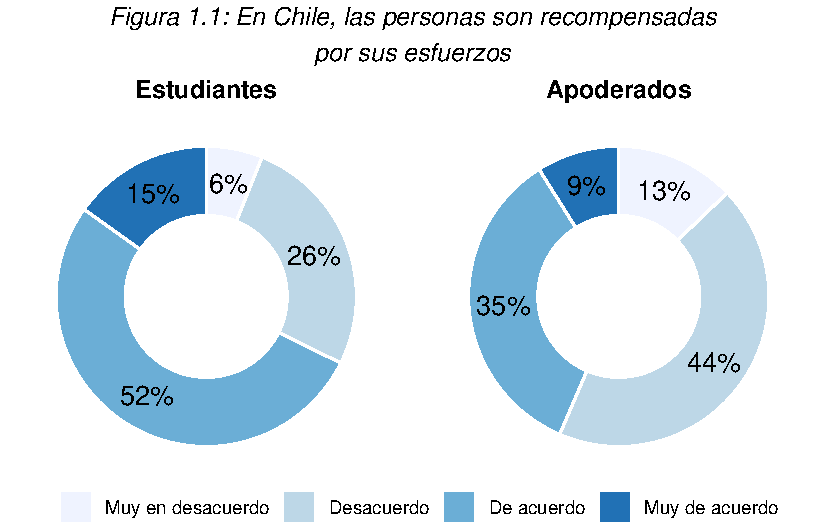
\includegraphics{meritocracia_files/figure-pdf/plot-esfuerzo-percep-1.pdf}

En primer lugar, se observan diferencias entre apoderados y estudiantes.
Los apoderados estan en desacuerdo con la frase. Así, los estudiantes
parecen estar más de acuerdo con que las personas en el país son
recompensadas por sus esfuerzos (52\%). Además, si se diferencia a los
estudiantes por curso, es posible observar que los estudiantes de
educación básica (80\%) están más de acuerdo que los estudiantes de
educación media (55\%).

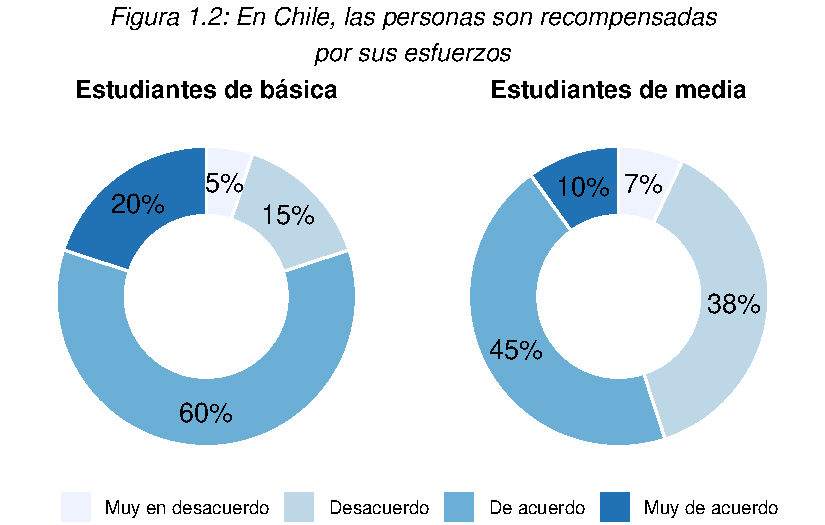
\includegraphics{meritocracia_files/figure-pdf/plot-esfuerzo-percep-curso-1.pdf}

\emph{Cruces con otras características sociodemográficas de estudiantes}

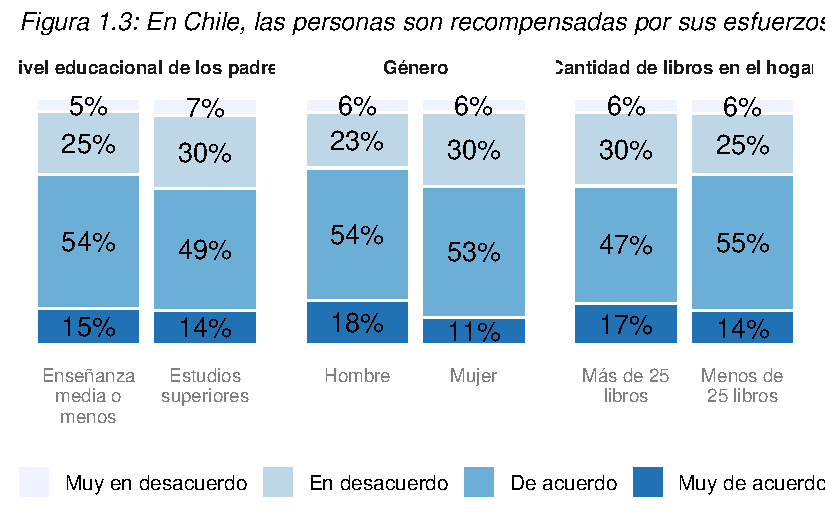
\includegraphics{meritocracia_files/figure-pdf/plot-esfuerzo-sociodemo-percep-1.pdf}

Estudiantes con padres que alcanzaron la enseñanza media o menos están
de acuerdo en un 54\% con la idea de que las personas son recompensadas
por sus esfuerzos en la sociedad. Diferenciando por género, mujeres
(53\%) y hombres (54\%) poseen porcentajes similares de acuerdo, a pesar
de ello se observa que estudiantes mujeres están mayormente en
desacuerdo con la frase (30\%) y estudiantes hombres consideran estar
muy de acuerdo con la frase en un 18\%. Estudiantes que poseen menos de
25 libros en su hogar estan más de acuerdo con que las personas son
recompensadas por sus esfuerzos en la sociedad (55\%). Sin embargo,
estudiantes con más de 25 libros consideran estar muy de acuerdo en un
17\% con la frase en comparación con los primeros que lo están en un
14\%.

\textbf{Talento} (inteligencia y habilidad) en la sociedad chilena:

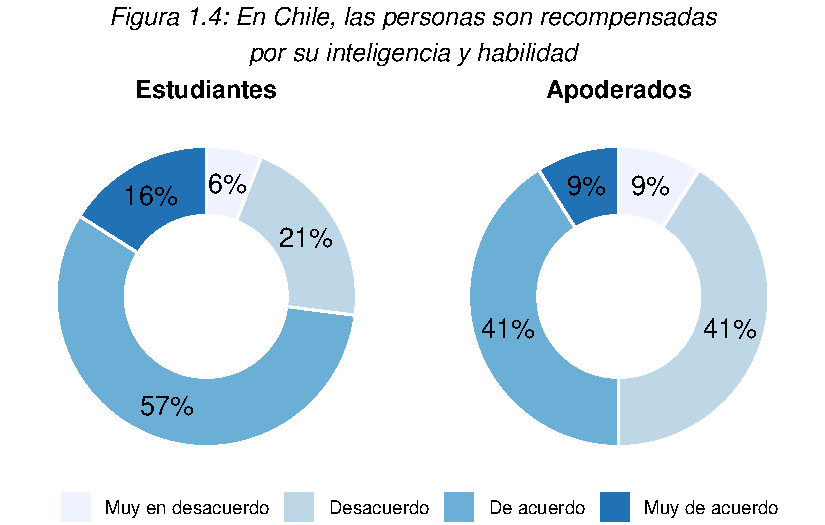
\includegraphics{meritocracia_files/figure-pdf/plot-talento-percep-1.pdf}

Estudiantes se muestran en su mayoría de acuerdo con la afirmación
(57\%). En cambio, los apoderados si bien tienen un gran porcentaje de
acuerdo con el talento, este es un 50\%. Por otro lado, estudiantes de
enseñanza báscia se muestran más de acuerdo con la idea de que el
talento es recompensado en la sociedad con un 76\%, considernado que se
encuentran un 20\% muy de acuerdo y un 56\% de acuerdo con la
afirmación.

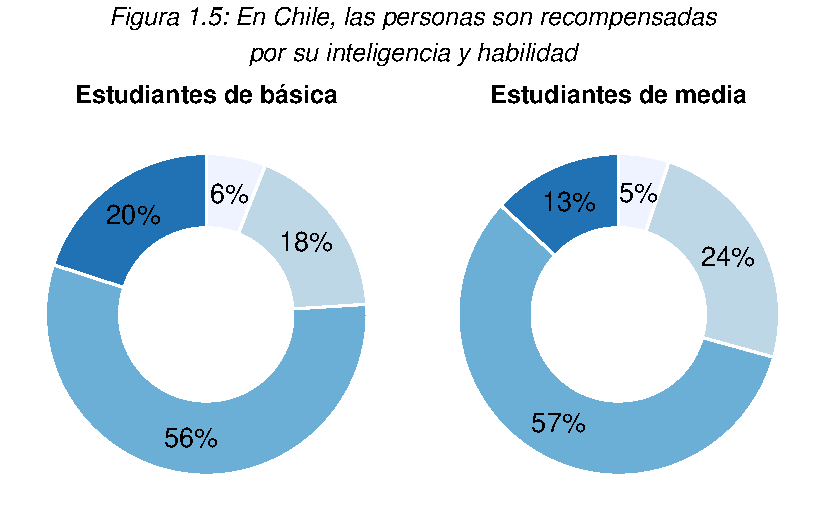
\includegraphics{meritocracia_files/figure-pdf/plot-talento-percep-curso-1.pdf}

\emph{Cruces con otras características sociodemográficas de estudiantes}

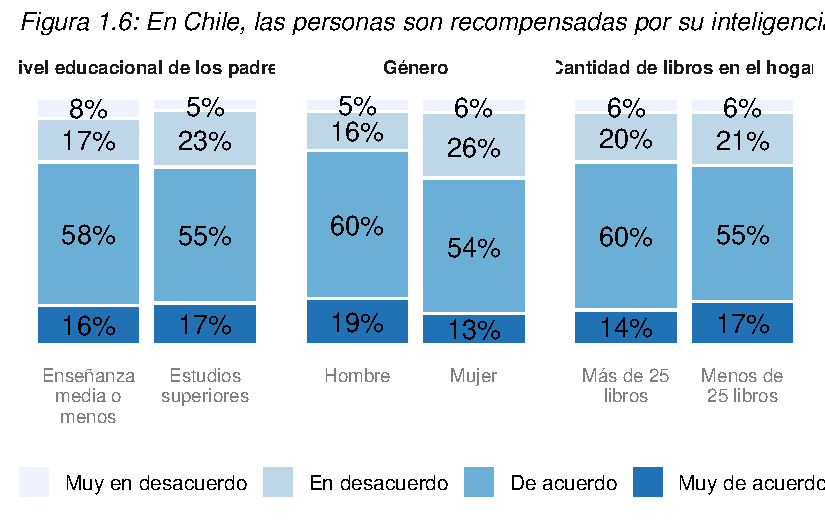
\includegraphics{meritocracia_files/figure-pdf/plot-talento-sociodemo-percep-1.pdf}

Estudiantes que tienen padres con estudios superiores se muestran en
desacuerdo con la frase en un 23\% a diferencia de quienes poseen padres
con enseñanza media o menos, quienes estan en desacuerdo en un 17\%. En
su mayoría, estos últimos se muestran de acuerdo en un 58\% con que las
personas son recompensadas por su inteligencia y habilidad en la
sociedad. Diferenciando por género, estudiantes hombres se muestran más
de acuerdo con la frase. Así, estos contestaron estar de acuerdo en un
60\% y muy de acuerdo en un 19\%. Estudiantes con más de 25 libros en su
hogar se muestran de acuerdo en un 60\% con la frase. A pesar de eso,
estudiantes con menos de 25 libros en su hogar se muestran muy de
acuerdo en un 17\%.

Respecto al \textbf{mérito} en la sociedad chilena:

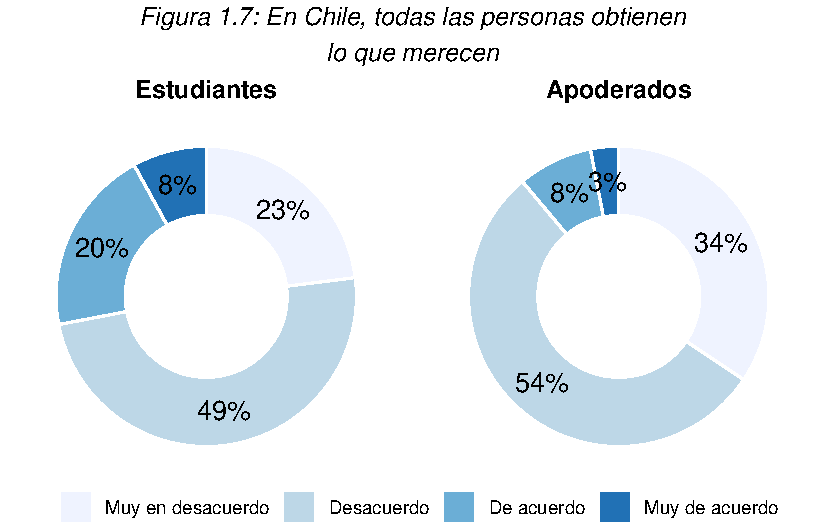
\includegraphics{meritocracia_files/figure-pdf/plot-merito-percep-1.pdf}

Si bien estudiantes y apoderados también se muestran en su mayoría en
desacuerdo con que todas las personas obtienen lo que merecen en la
sociedad, los estudiantes presentan un 20\% de acuerdo con la
afirmación. Respecto al curso de estos, específicamente estudiantes de
básica contestaron estar de acuerdo en un 24\% y muy de acuerdo en un
13\%.

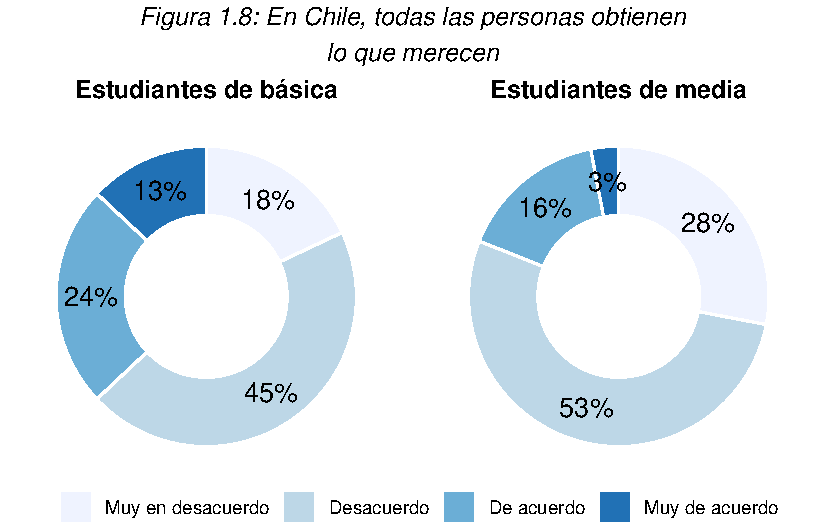
\includegraphics{meritocracia_files/figure-pdf/plot-merito-percep-curso-1.pdf}

\emph{Cruces con características sociodemográficas de estudiantes}

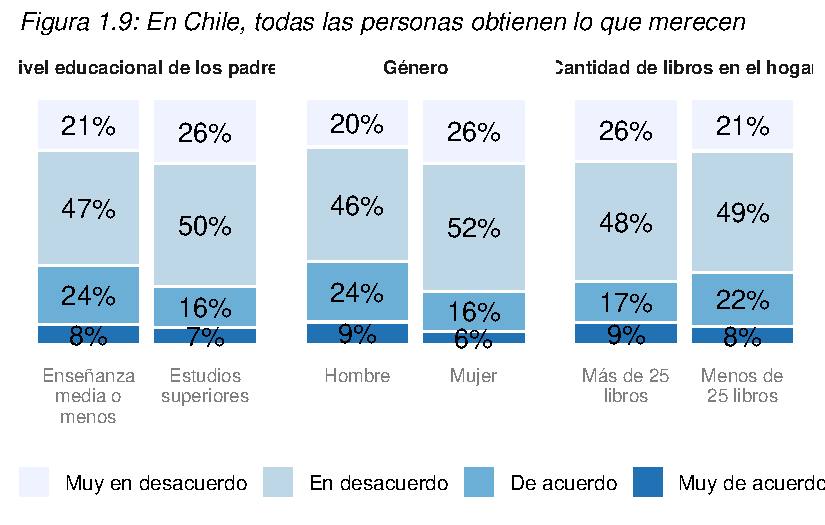
\includegraphics{meritocracia_files/figure-pdf/plot-merito-sociodemo-percep-1.pdf}

Estudiantes con padres que tienen estudios superiores estan en
desacuerdo en un 50\% y muy en desacuerdo en un 26\% con que todas las
personas obtienen lo que merecen en la sociedad. Diferenciando por
género, mujeres están en desacuerdo en un 52\% con la frase. Estudiantes
con más de 25 libros en su hogar estan muy en desacuerdo en un 26\% y en
desacuerdo en un 48\%.

\begin{itemize}
\tightlist
\item
  Respecto a factores no meritocráticos
\end{itemize}

Estos factores aluden a externalidades del mérito individual como la
herencia, los contactos y la suerte. Por ello, se presentan preguntas
referidas a la percepción respecto a los logros individuales de las
personas que tienen padres ricos, buenos contactos y mejores
oportunidades en la vida.

\textbf{Padres ricos} y logro indiviudal en la sociedad chilena:

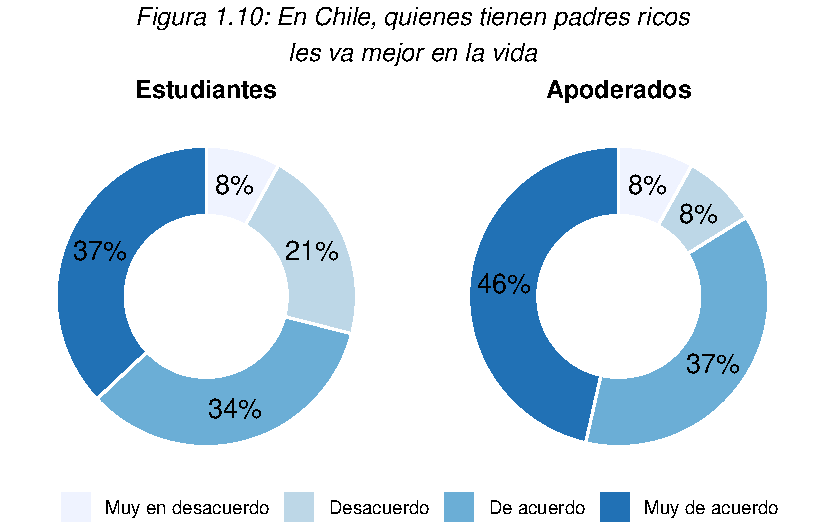
\includegraphics{meritocracia_files/figure-pdf/plot-padres-ricos-percep-1.pdf}

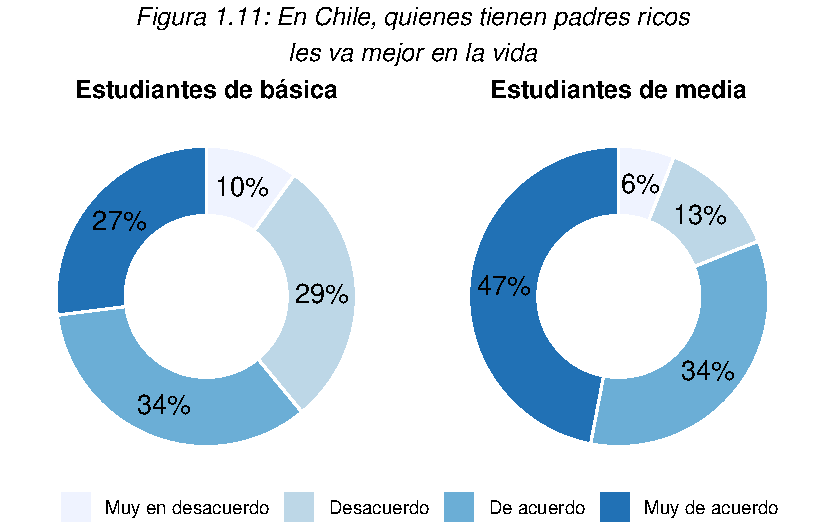
\includegraphics{meritocracia_files/figure-pdf/plot-padres-ricos-percep-curso-1.pdf}

\emph{Cruces con características sociodemográficas de estudiantes}

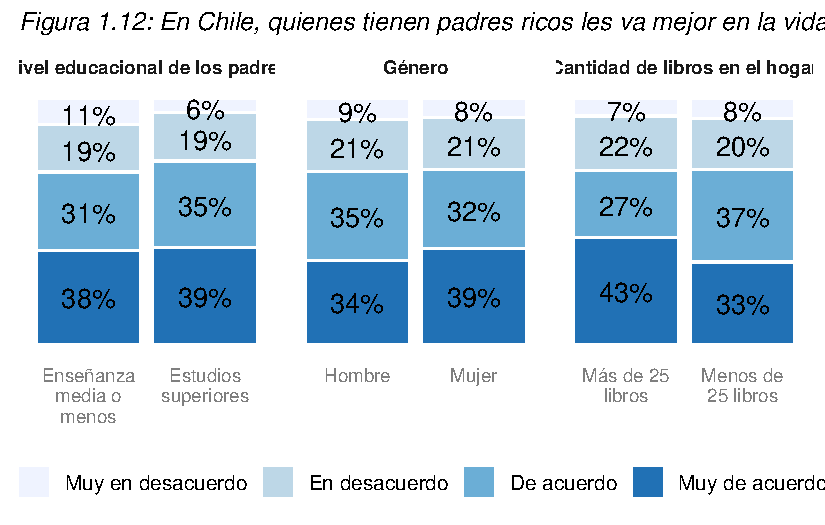
\includegraphics{meritocracia_files/figure-pdf/plot-padres-ricos-sociodemo-percep-1.pdf}

\textbf{Buenos contactos} y logro individual en la sociedad chilena:

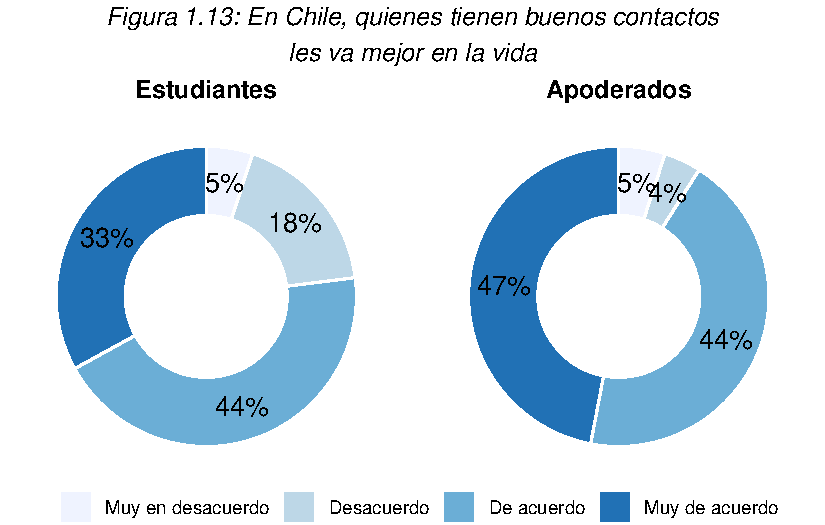
\includegraphics{meritocracia_files/figure-pdf/plot-buenos-contactos-percep-1.pdf}

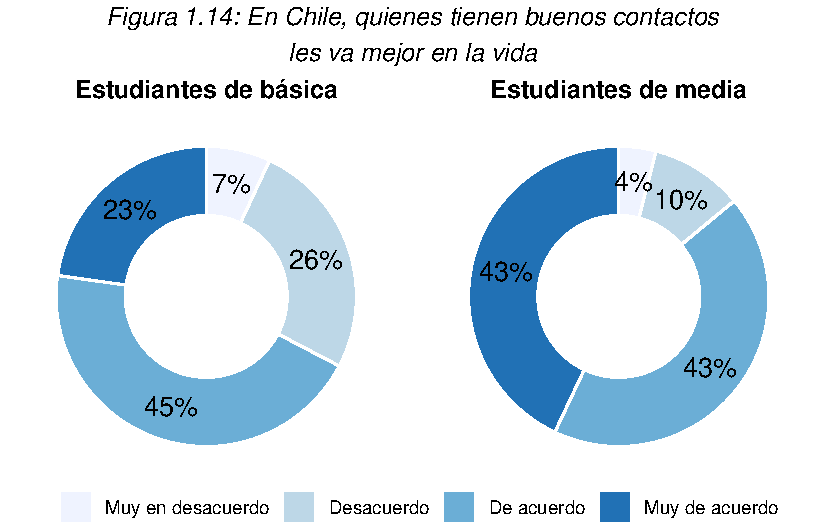
\includegraphics{meritocracia_files/figure-pdf/plot-buenos-contactos-percep-curso-1.pdf}

\emph{Cruce con características sociodemográficas}

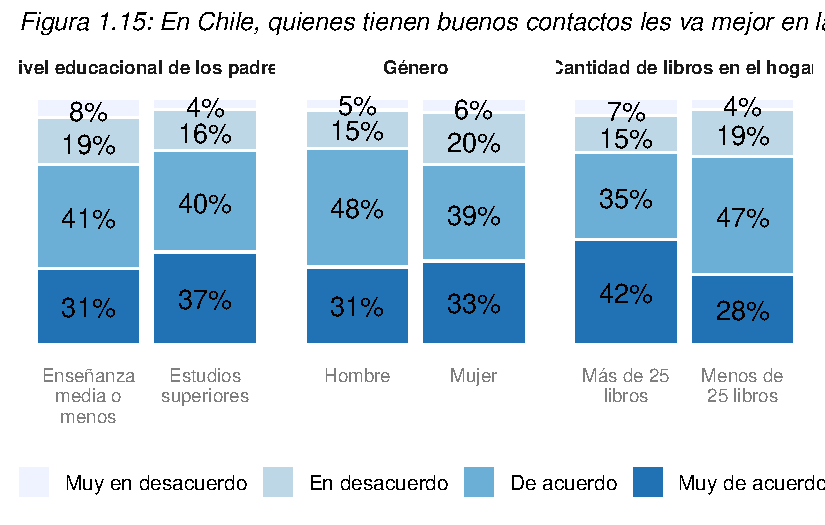
\includegraphics{meritocracia_files/figure-pdf/plot-buenos-contactos-sociodemo-percep-1.pdf}

\textbf{Oportunidades} y logro individual en la sociedad chilena:

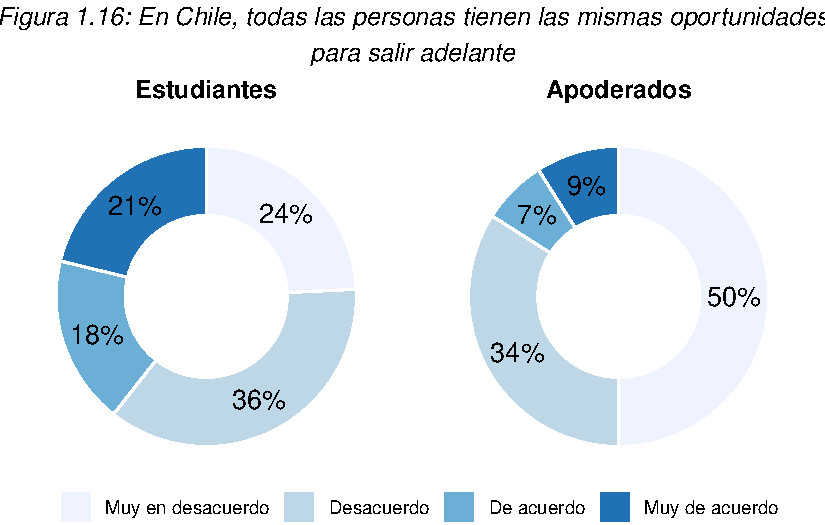
\includegraphics{meritocracia_files/figure-pdf/plot-oportunidades-1.pdf}

Descripción\ldots..

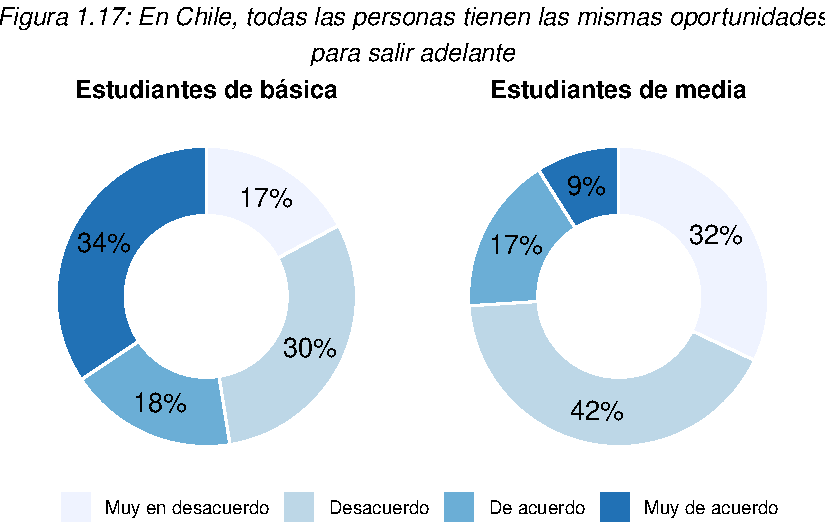
\includegraphics{meritocracia_files/figure-pdf/plot-oportunidades-curso-1.pdf}

\emph{Cruces con características sociodemográficas de estudiantes}

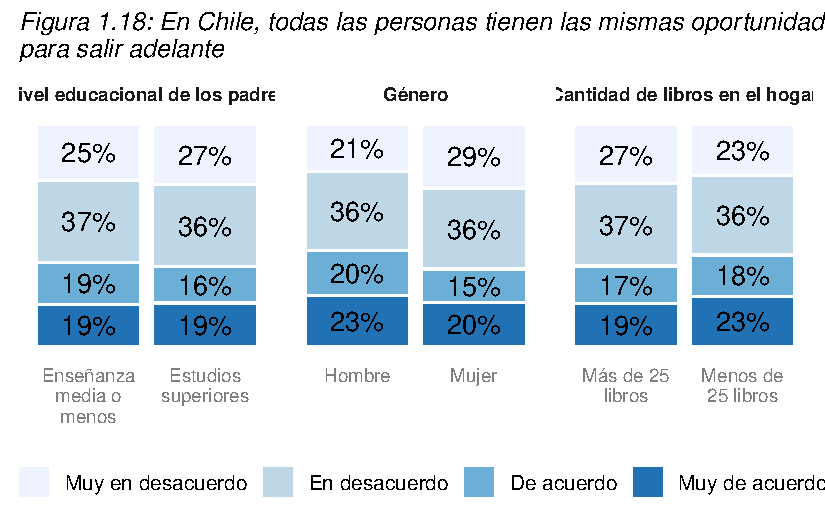
\includegraphics{meritocracia_files/figure-pdf/plot-oportunidades-sociodemo-1.pdf}

\subsubsection{Preferencias}\label{preferencias}

\begin{itemize}
\tightlist
\item
  Respecto a criterios de mérito individual
\end{itemize}

\textbf{Esfuerzo} en la sociedad chilena:

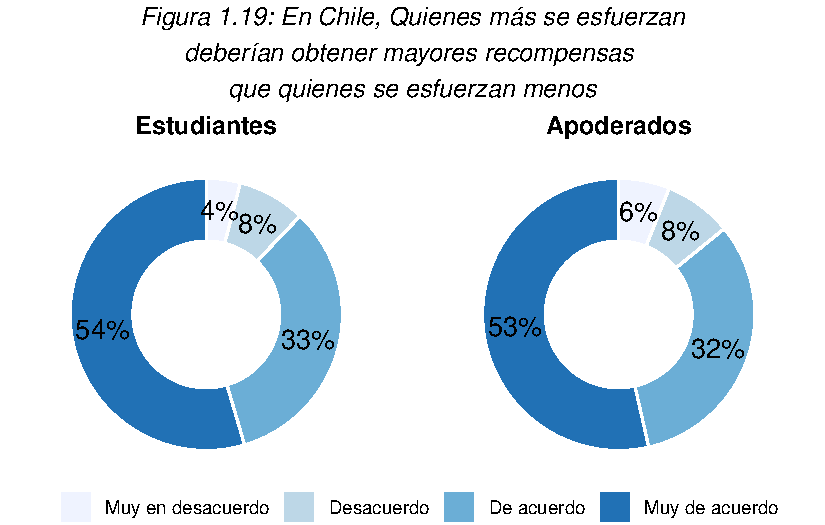
\includegraphics{meritocracia_files/figure-pdf/plot-esfuerzo-pref-1.pdf}

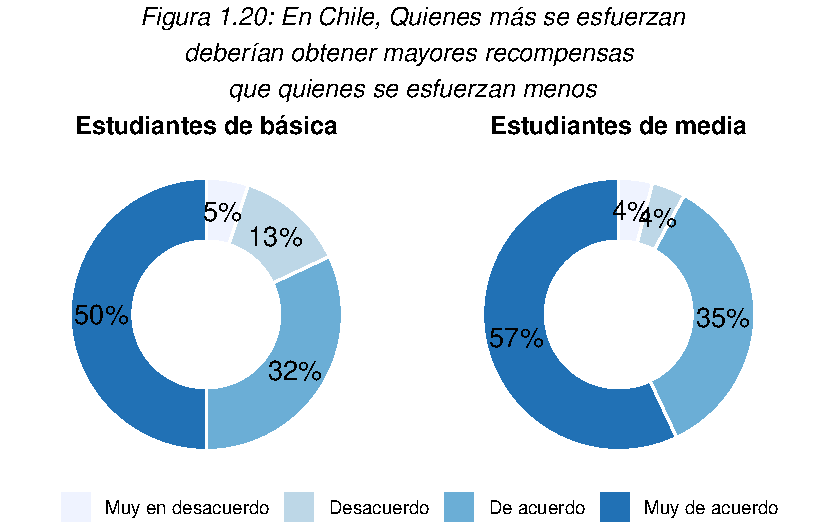
\includegraphics{meritocracia_files/figure-pdf/plot-esfuerzo-pref-curso-1.pdf}

\emph{Cruces con características sociodemográficas de estudiantes}

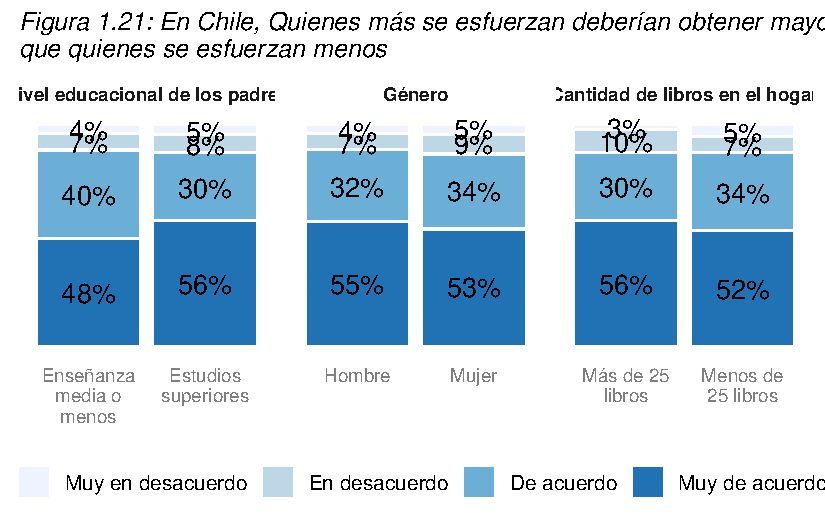
\includegraphics{meritocracia_files/figure-pdf/plot-esfuerzo-pref-sociodemo-1.pdf}

\textbf{Talento} en la sociedad chilena:

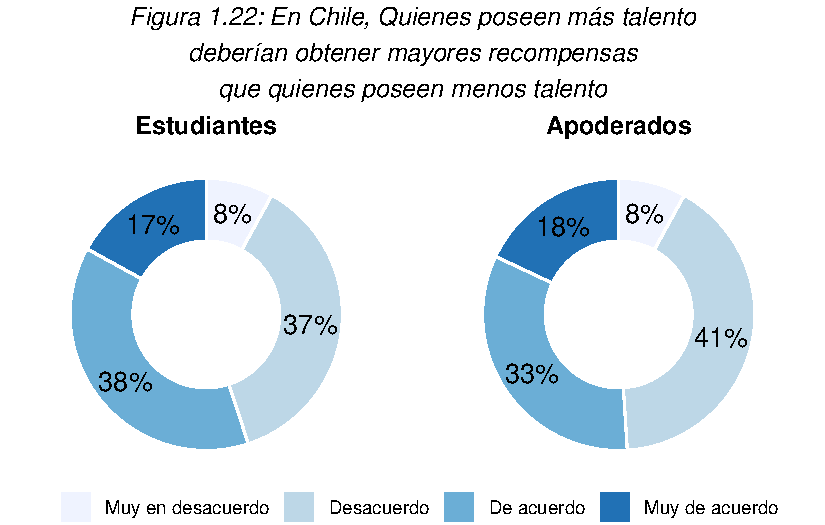
\includegraphics{meritocracia_files/figure-pdf/plot-talento-pref-1.pdf}

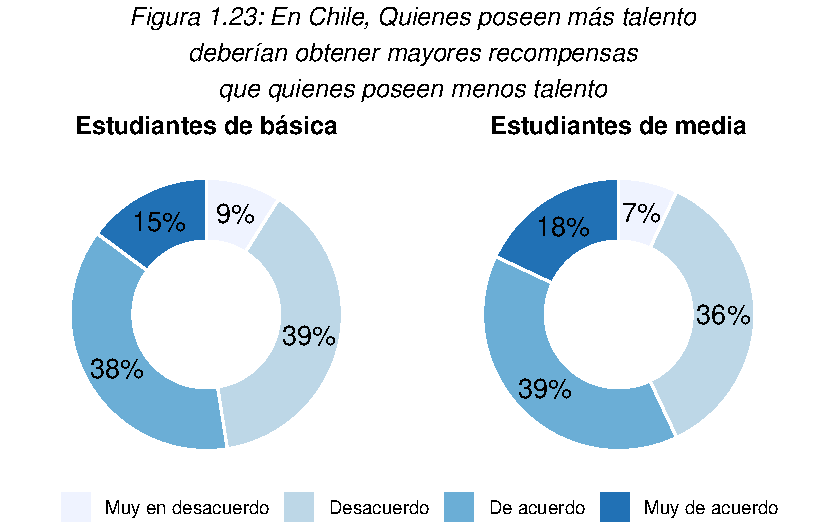
\includegraphics{meritocracia_files/figure-pdf/plot-talento-pref-curso-1.pdf}

\emph{Cruces con características sociodemográficas de estudiantes}

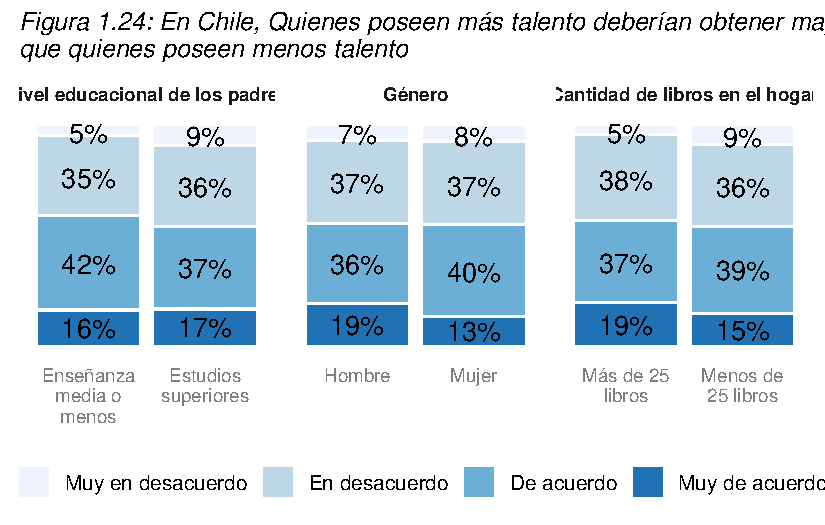
\includegraphics{meritocracia_files/figure-pdf/plot-talento-pref-sociodemo-1.pdf}

\begin{itemize}
\tightlist
\item
  Preferencia respecto a la recompensa en base al talento por sobre el
  esfuerzo
\end{itemize}

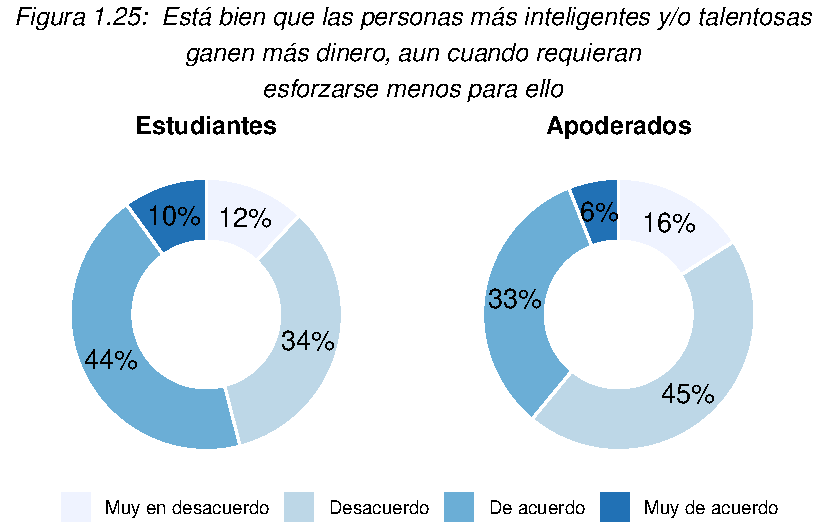
\includegraphics{meritocracia_files/figure-pdf/plot-merito-pref-1.pdf}

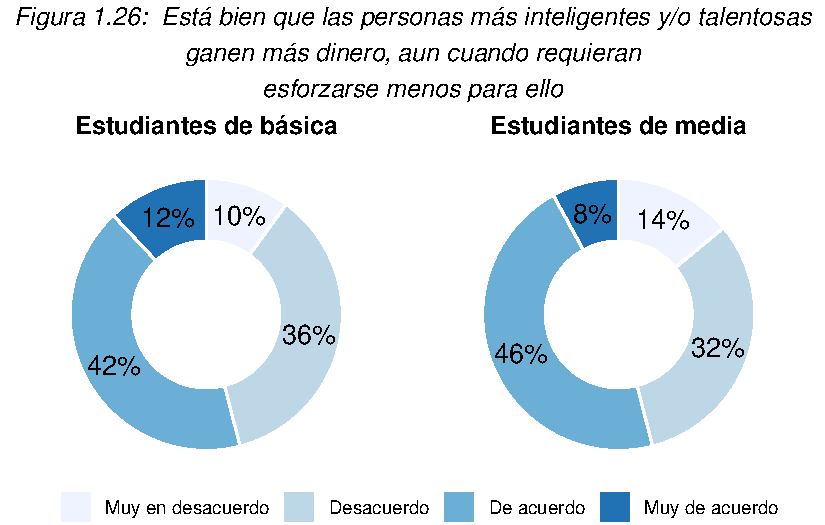
\includegraphics{meritocracia_files/figure-pdf/plot-merito-pref-curso-1.pdf}

\emph{Cruces con características sociodemográficas de estudiantes}

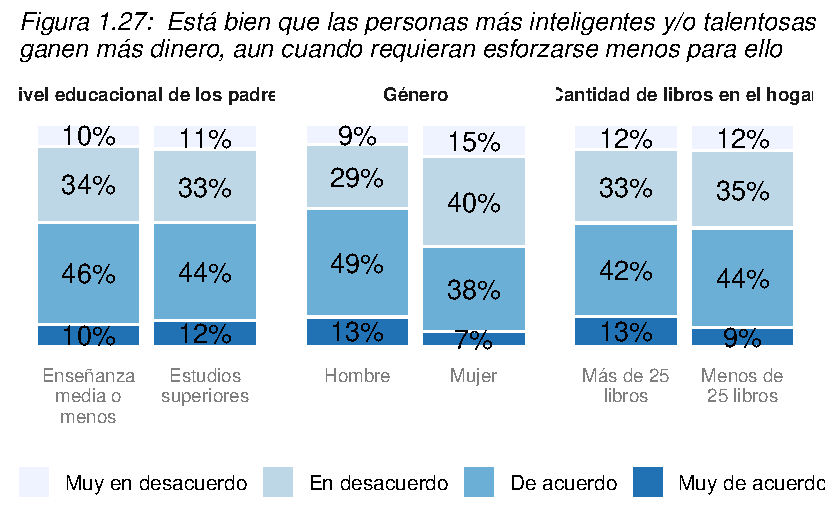
\includegraphics{meritocracia_files/figure-pdf/plot-merito-pref-sociodemo-1.pdf}

\begin{itemize}
\tightlist
\item
  Respecto a factores no meritocráticos
\end{itemize}

Estos factores aluden a externalidades del mérito individual como la
herencia, los contactos y la suerte. Por ello, se presentan preguntas
referidas a la preferencia respecto a los logros individuales de las
personas que tienen padres ricos, buenos contactos.

\textbf{Padres ricos}

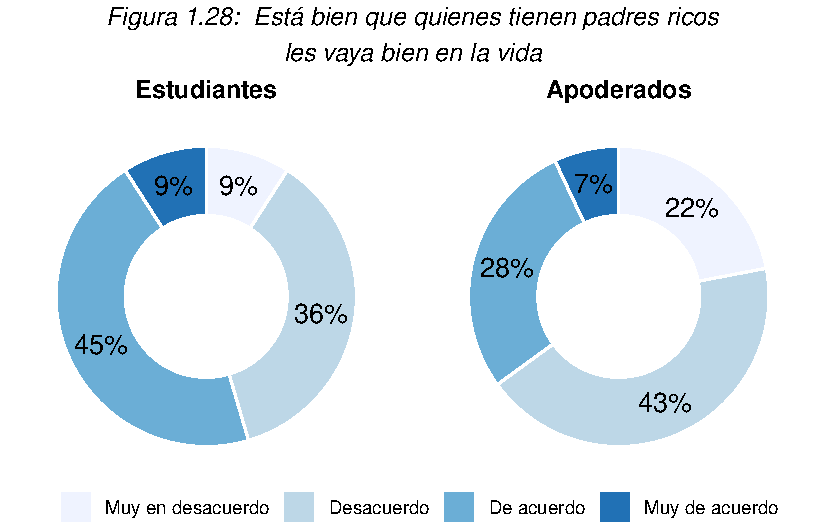
\includegraphics{meritocracia_files/figure-pdf/plot-padres-ricos-pref-1.pdf}

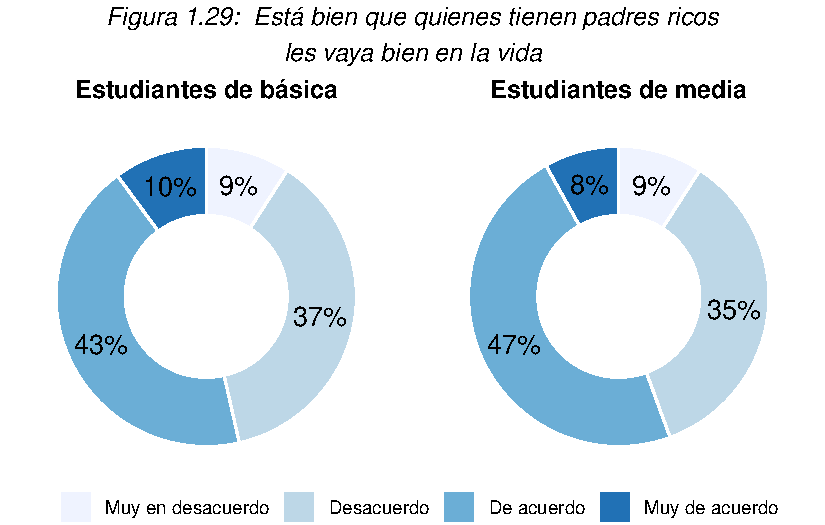
\includegraphics{meritocracia_files/figure-pdf/plot-padres-ricos-pref-curso-1.pdf}

\emph{Cruces con características sociodemográficas de estudiantes}

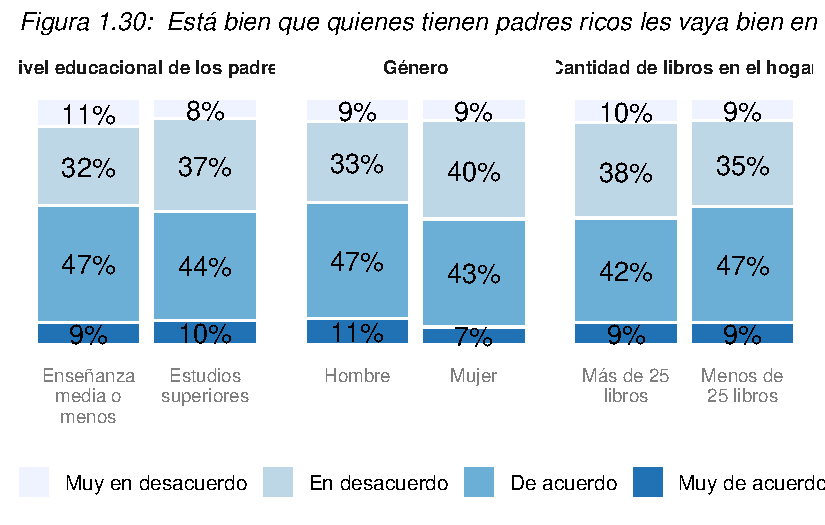
\includegraphics{meritocracia_files/figure-pdf/plot-padres-ricos-pref-sociodemo-1.pdf}

\textbf{Buenos contactos}

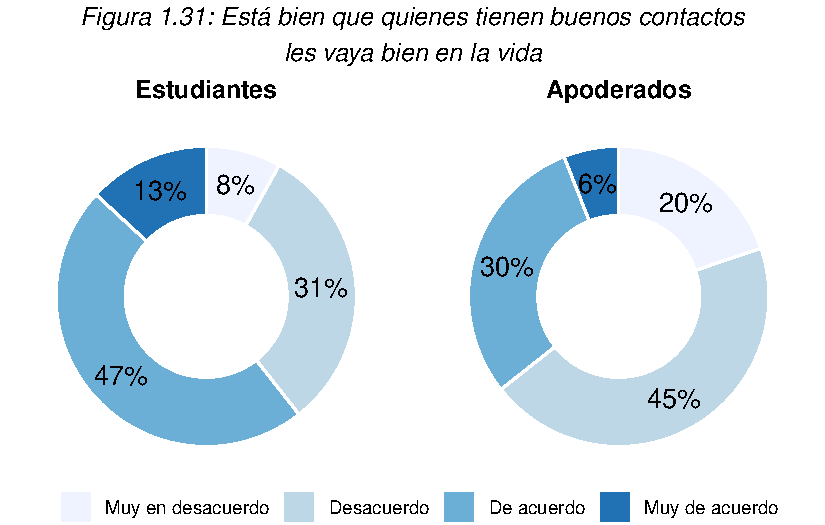
\includegraphics{meritocracia_files/figure-pdf/plot-buenos-contactos-pref-1.pdf}

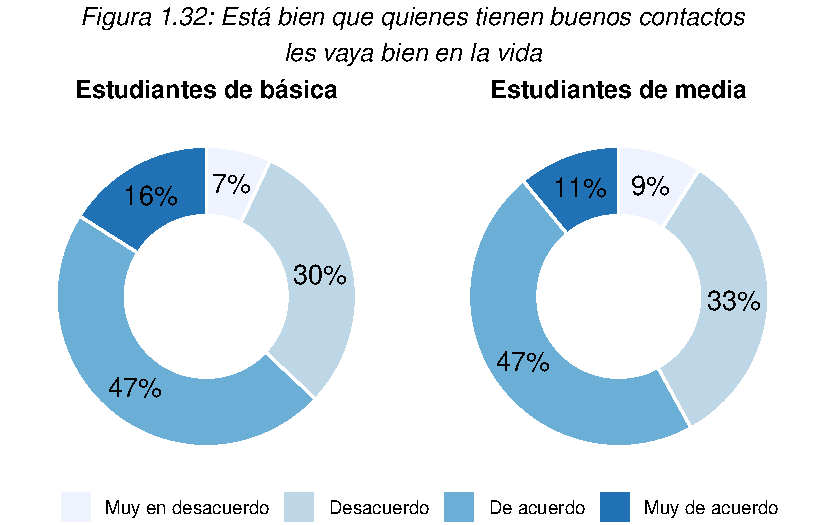
\includegraphics{meritocracia_files/figure-pdf/plot-buenos-contactos-pref-curso-1.pdf}

\emph{Cruces con características sociodemográficas de estudiantes}

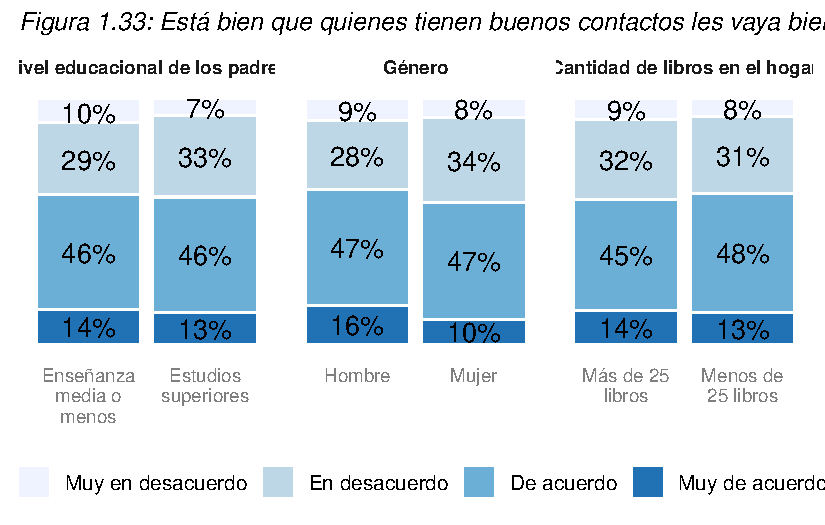
\includegraphics{meritocracia_files/figure-pdf/plot-buenos-contactos-pref-sociodemo-1.pdf}

\section{Meritocracia en la escuela}\label{meritocracia-en-la-escuela}

En este módulo se considera otro apartado adicional a las creencias de
las/los estudiantes, el que está referido a la experiencia de estas
mismas/mismos en sus notas. La forma en que se estudia la meritocracia
escolar a partir de la experiencia en la nota se evidencia en la idea de
que el mérito de ellas/ellos sea justamente reconocido en la nota
obtenida. Por esa razón, dicho apartado se denominará ``justicia en las
notas''.

De este modo, se presentan dos apartados: \textbf{creencias en la
meritocracia} y \textbf{justicia en las notas}.

\subsection{Creencias en la
meritocracia}\label{creencias-en-la-meritocracia-1}

\subsubsection{Percepciones}\label{percepciones-1}

\begin{itemize}
\tightlist
\item
  Respecto a criterios de mérito individual
\end{itemize}

\textbf{Esfuerzo} en la escuela:

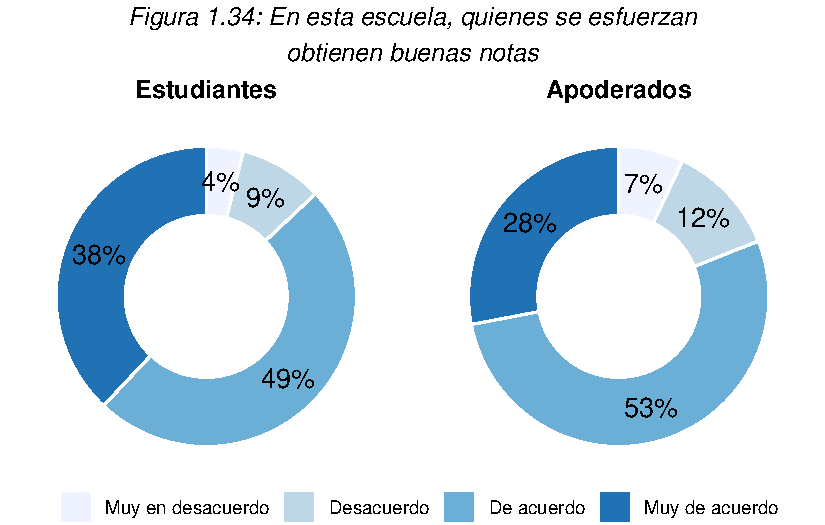
\includegraphics{meritocracia_files/figure-pdf/plot-school-esfuerzo-1.pdf}

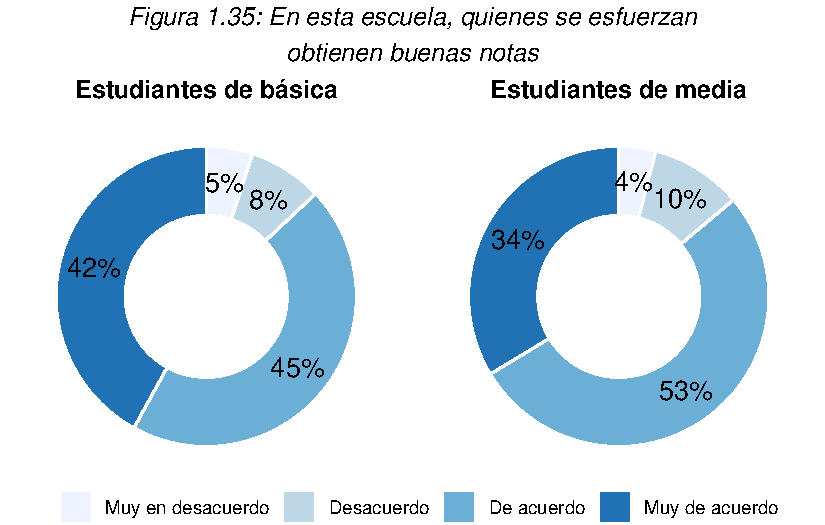
\includegraphics{meritocracia_files/figure-pdf/plot-school-esfuerzo-curso-1.pdf}

\emph{Cruces con características sociodemográficas de estudiantes}

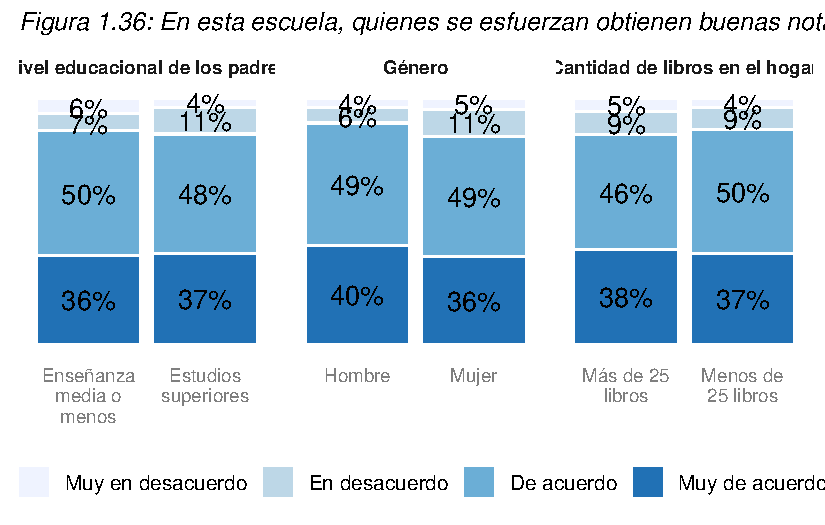
\includegraphics{meritocracia_files/figure-pdf/plot-school-esfuerzo-sociodemo-1.pdf}

\textbf{Talento} en la escuela:

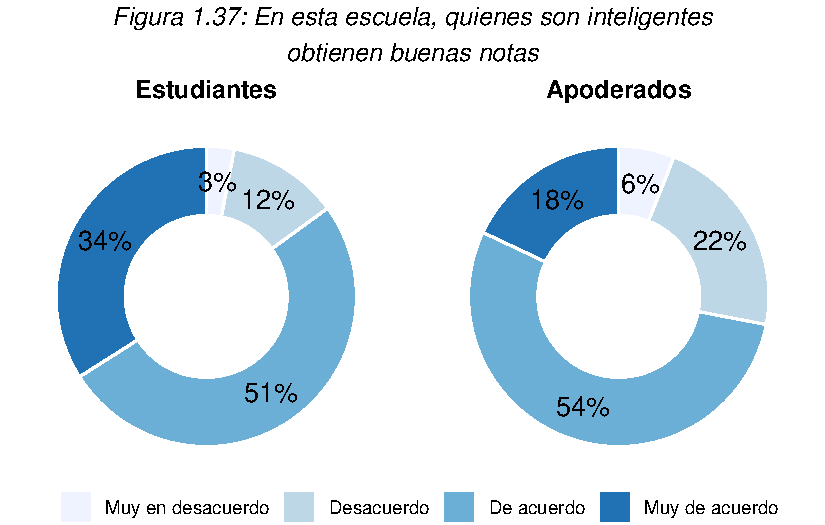
\includegraphics{meritocracia_files/figure-pdf/plot-school-talento-1.pdf}

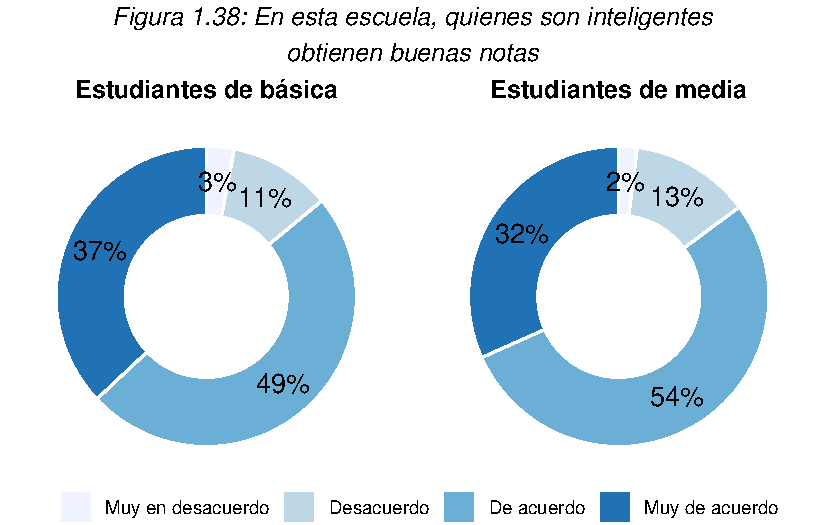
\includegraphics{meritocracia_files/figure-pdf/plot-school-talento-curso-1.pdf}

\emph{Cruces con características sociodemográficas de estudiantes}

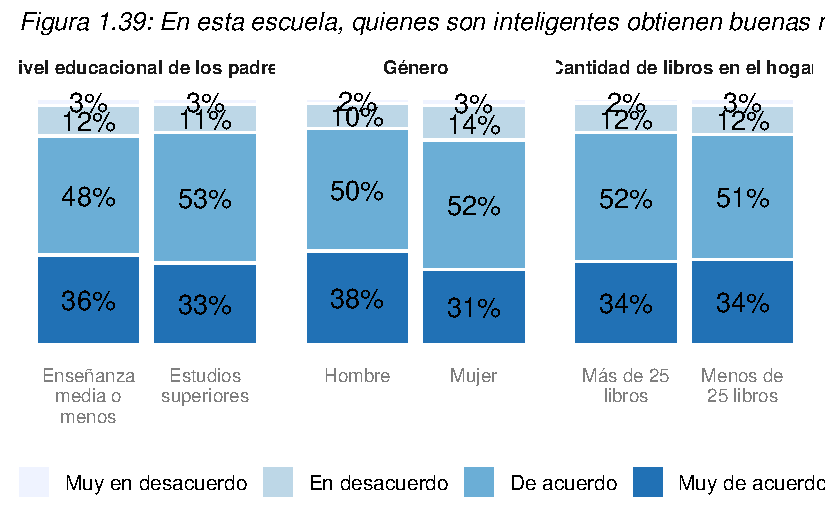
\includegraphics{meritocracia_files/figure-pdf/plot-school-talento-sociodemo-1.pdf}

Respecto al~\textbf{mérito}~en la escuela:

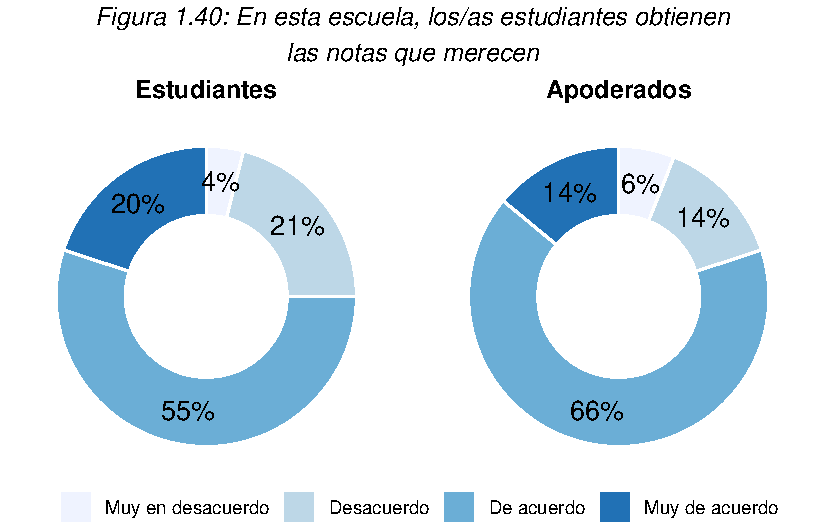
\includegraphics{meritocracia_files/figure-pdf/plot-school-merito-1.pdf}

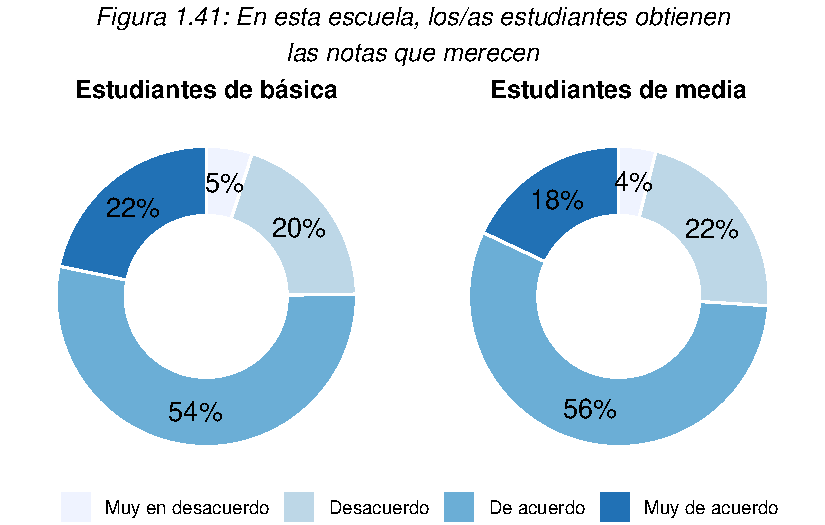
\includegraphics{meritocracia_files/figure-pdf/plot-school-merito-curso-1.pdf}

\emph{Cruces con características sociodemográficas de estudiantes}

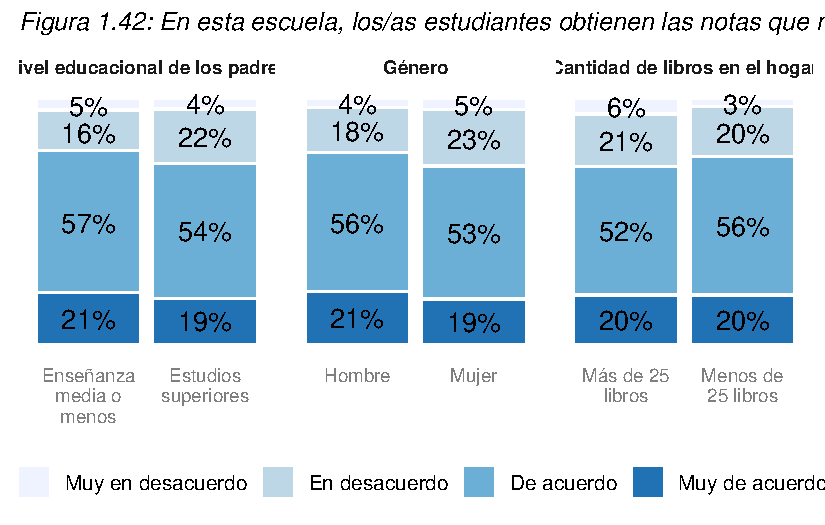
\includegraphics{meritocracia_files/figure-pdf/plot-school-merito-sociodemo-1.pdf}

\subsubsection{Preferencia}\label{preferencia}

\begin{itemize}
\tightlist
\item
  Respecto a criterios de mérito individual:
\end{itemize}

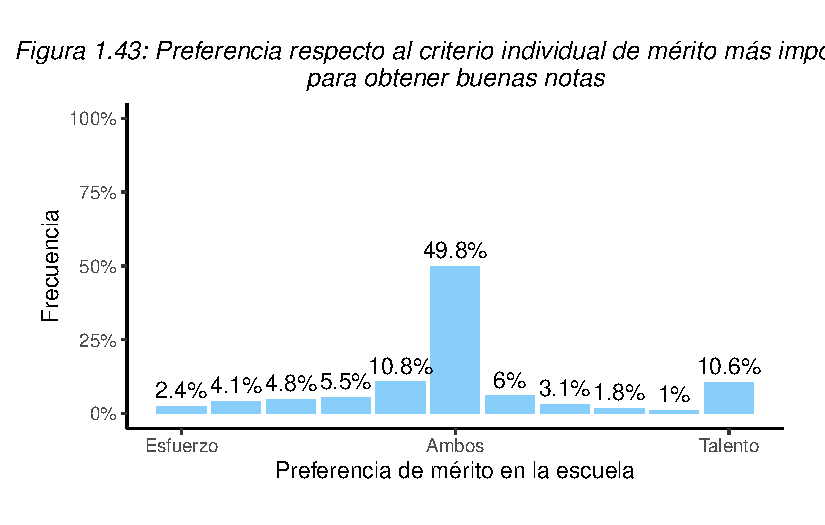
\includegraphics{meritocracia_files/figure-pdf/plot-school-pref-1.pdf}

Los estudiantes consideran que ambos criterios individuales son
importantes para obtener buenas notas en la escuela con un 49\%.
Particularmente, se observa que un 10\% cree que el talento es relevante
y el 2\% considera que el esfuerzo es importante para la obtención de
buenas calficaciones.

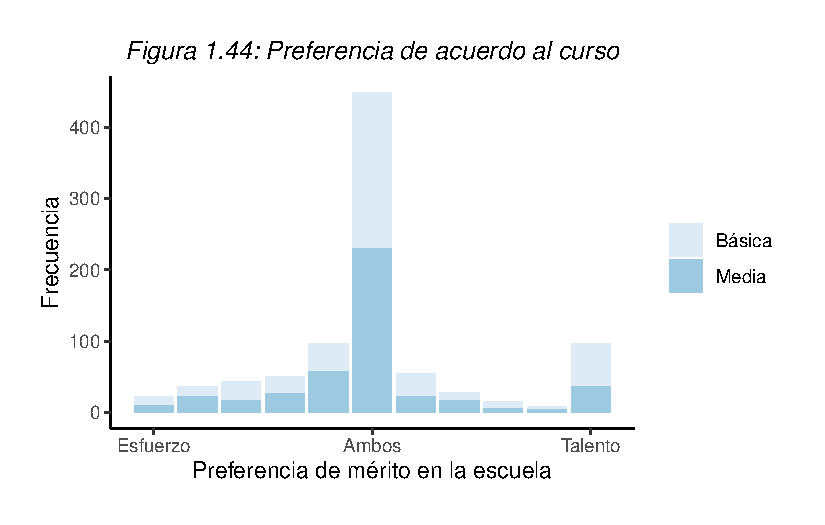
\includegraphics{meritocracia_files/figure-pdf/plot-school-pref-curso-1.pdf}

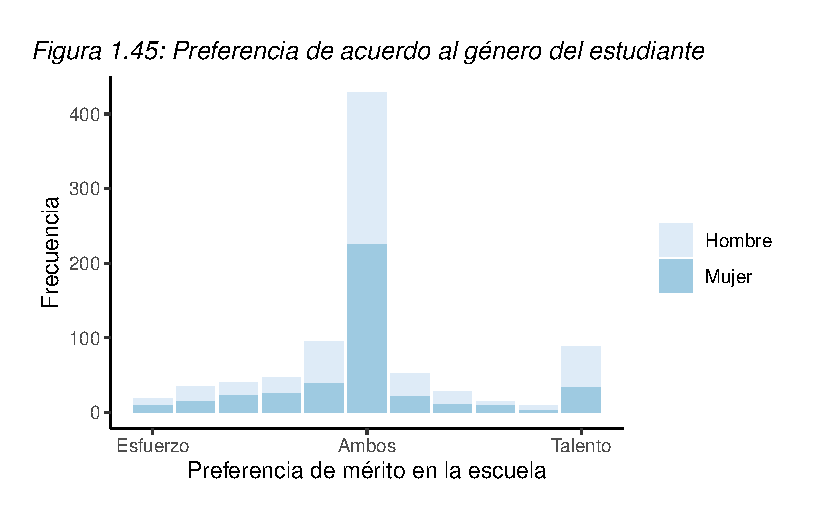
\includegraphics{meritocracia_files/figure-pdf/plot-school-pref-gen-1.pdf}

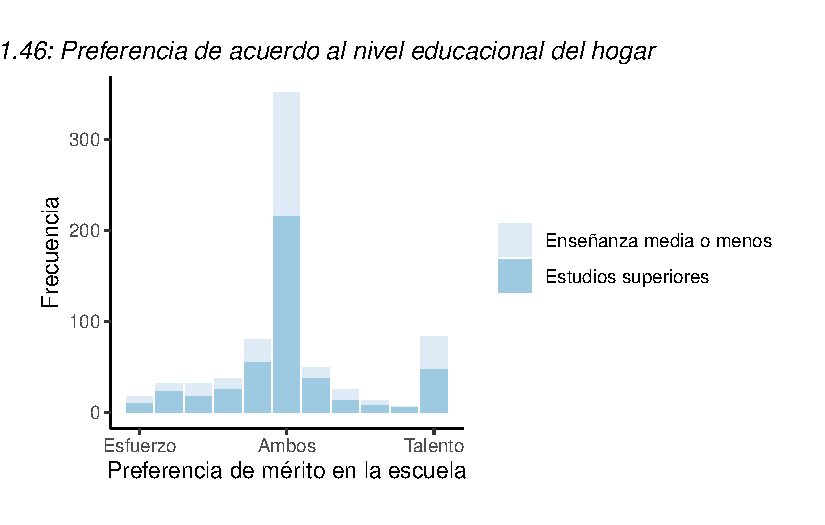
\includegraphics{meritocracia_files/figure-pdf/plot-school-pref-ne-1.pdf}

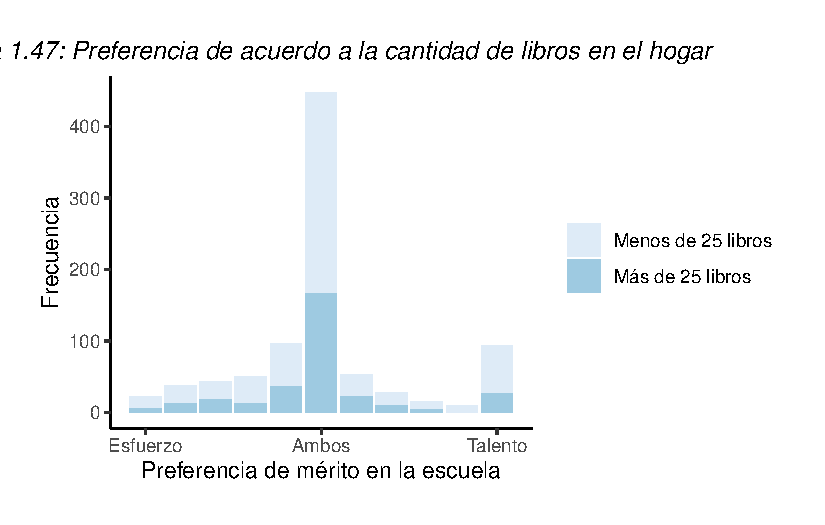
\includegraphics{meritocracia_files/figure-pdf/plot-school-pref-libros-1.pdf}

\subsection{Justicia en las notas}\label{justicia-en-las-notas}

En este apartado se observa la percepción de las/los estudiantes
respecto a si la nota obtenida recompensa de manera justa su mérito
individual. Posteriormente, se presenta de manera comparativa la nota
que efectivamente estos recibieron y la preferencia que ellas/ellos
tenían de la nota que debieron haber obtenido.

\subsubsection{Percepciones}\label{percepciones-2}

\emph{a. Respecto a la justicia de la nota obtenida}

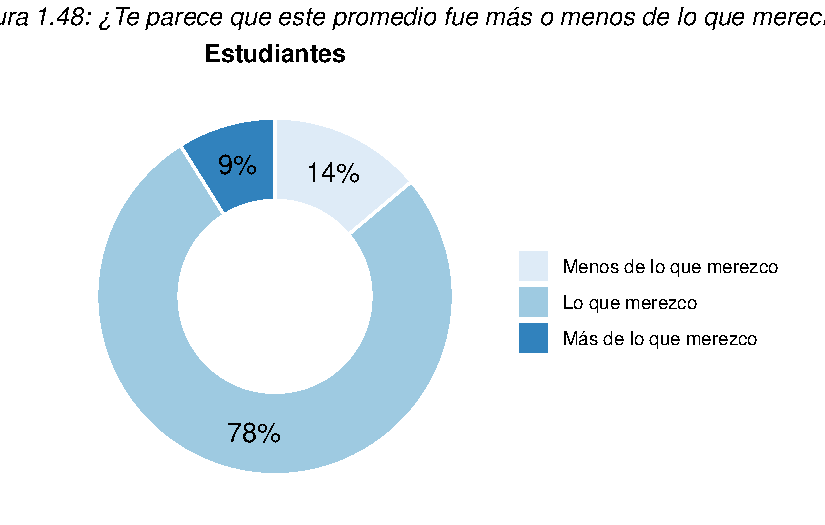
\includegraphics{meritocracia_files/figure-pdf/plot-notas-merit-1.pdf}

Los estudiantes

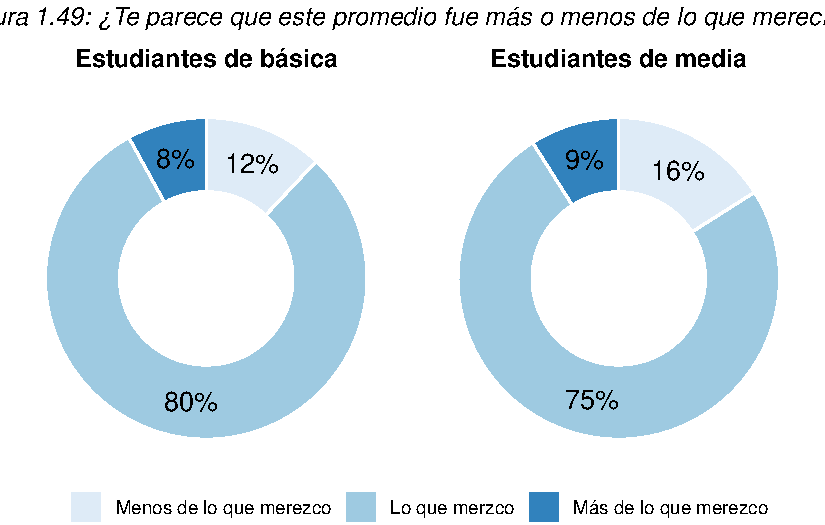
\includegraphics{meritocracia_files/figure-pdf/plot-notas-merit-curso-1.pdf}

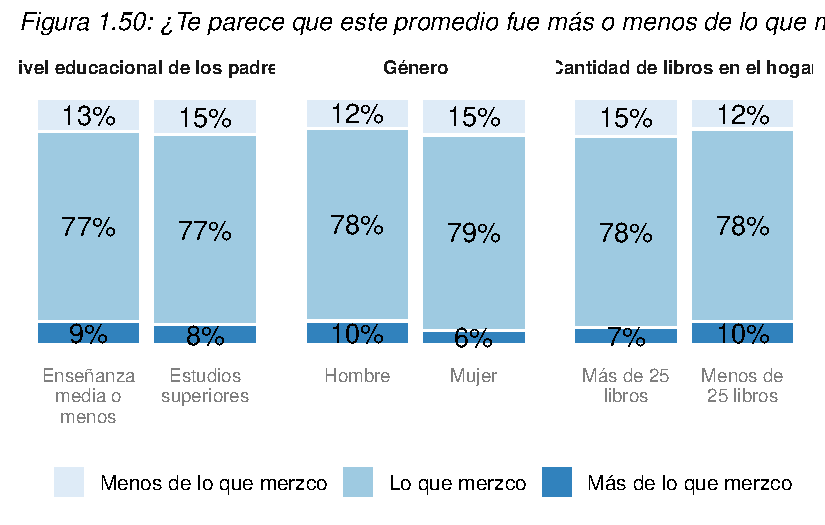
\includegraphics{meritocracia_files/figure-pdf/plot-notas-merit-sociodemo-1.pdf}

\includegraphics{meritocracia_files/figure-pdf/plot-notas-esfuerzo-1.pdf}

Los estudiantes consideran en un 78\% que el promedio obtenido el año
pasado es el que merecían, por ende, sus méritos son recompensados en su
nota obtenida. Además, contestaron en un 71\% que dichas notas son las
que estos merecían de acuerdo al tiempo que le dedican a sus estudios,
en ese sentido, su esfuerzo se ve recompensado en esa nota.

\includegraphics{meritocracia_files/figure-pdf/plot-notas-esfuerzo-curso-1.pdf}

\includegraphics{meritocracia_files/figure-pdf/plot-notas-esfuerzo-sociodemo-1.pdf}

\subsubsection{Notas del estudiante}\label{notas-del-estudiante}

Este apartado hace énfasis en la nota individual de la/el estudiante. De
ese modo, se presenta comparativamente la \emph{nota final que
efectivamente obtuvo} y la \emph{nota final que consideraba que debería
haber obtenido}. Además, se realizan cruces para evidenciar como se
distribuye la percepción de merecimiento descrita en el apartado
anterior a partir de la nota obtenida del estudiante.

\includegraphics{meritocracia_files/figure-pdf/plot-just-nota-1.pdf}

En primera instancia, se puede observar que los estudiantes que se
sienten subrecompensados con su nota tienden a preferir en mayor medida
notas superiores a 5,0. Además, se observa un contraste entre una gran
cantidad de estudiantes que preferían una nota 7,0 o cercana a la nota
máxima, y quienes obtuvieron efectivamente esa nota. Para los
estudiantes que se sintieron sobrerecompensados, se observa un contraste
entre la nota obtenida y la nota que creen merecer en torno a las notas
cercanas al 4,0 y 5,0. Así, estos estudiantes obtuvieron en mayor medida
notas entre 6,0 y menor a 7,0, creyendo merecer notas entre el 4.0 y el
6,0.

\bookmarksetup{startatroot}

\chapter{Ciudadanía}\label{ciudadanuxeda}

La idea de ciudadanía se entiende a partir de dos dimensiones: cívica y
civil. Esta se encuentra orientada a la idea de participación en la
sociedad, en tanto aspectos políticos formales como proyectos colectivos
de acción social y aspectos de convivencia que son entendidos como
prosociales. Ambos tipos pretenden aportar a la cohesión de las
sociedades cuando se ejerce dicha participación ciudadana. Así, esas
características de participación se posicionan como un ideal normativo
enmarcado en la idea de buena ciudadanía.

La escuela como espacio de socialización política aporta en dicha
formación de ciudadanía en los estudiantes. Lo anterior, se produce a
partir de los Planes de Formación Ciudadana que se encuentran presentes
en los curriculos escolares de los establecimientos. Con ello, el aula y
las prácticas pedagogicas son esenciales para la reproducción de las
ideas de ciudadanía que refieren al funcionamiento de la sociedad y la
democracia.

Adicionalmente, se reconoce otro espacio de socialización política y que
se consolida como el primer momento en que los niños/as son socializados
respecto a los criterios de buena ciudadanía: la familia. De ese modo,
el hogar es fundamental como primer espacio de acercamiento a las ideas
sobre la política.

Con aquello presente, este módulo se estrcutrará en cuatro grandes
apartados: \textbf{Formación ciudadana en la escuela},
\textbf{Participación política}, \textbf{Buena ciudadanía} y
\textbf{Relación con el adulto en el hogar}. Dentro de cada uno se
presentarán diversas preguntas referidas a actitudes y participación
para medir la ciudadanía en torno a las percepciones de los estudiantes
sobre criterios posicionados tanto a nivel del espacio escolar como en
la sociedad.

\section{Formación ciudadana en la
escuela}\label{formaciuxf3n-ciudadana-en-la-escuela}

En este primer apartado se presentan dos secciones: percepción de
importancia del establecimiento y dinámicas del proceso formativo por
parte del docente en el aula.

\subsection{Percepción respecto a la importancia que le entrega la
escuela}\label{percepciuxf3n-respecto-a-la-importancia-que-le-entrega-la-escuela}

Esta sección presenta una pregunta inicial referida al involucramiento
de la escuela con la Formación Ciudadana. En ese sentido, la pregunta
alude a la importancia que los estudiantes consideran que le entrega el
establecimiento a la educación cívica en el espacio escolar.

\includegraphics{ciudadania_files/figure-pdf/plot-importancia-ciudadania-1.pdf}

En general, los estudiantes consideran que se le da una mediana
importancia a la Formación Ciudadana en la escuela. Particularmente ,los
estudiantes de enseñanza báscia consideran que se le da más importnacia,
contestando en un 29\% que la escuela le entrega mucha importancia,
encompración con los estudiantes de media (20\%).

\includegraphics{ciudadania_files/figure-pdf/plot-importancia-ciudadania-curso-1.pdf}

\subsection{En el espacio de clases}\label{en-el-espacio-de-clases}

Las preguntas de esta sección se enfocan en la dinámica de interacción
entre docente y estudiantes en el aula. Específicamente, estas son
referidas al momento en que se discute un tema político y social durante
la clase, aludiendo así al rol del docente en el proceso formativo.

\includegraphics{ciudadania_files/figure-pdf/plot-clases-ES-1.pdf}

Dentro de la dinámica en que los estudiantes plantean hechos políticos
de actualidad para discutir en la clase predomina la categoría casi
nunca con un 36\% y nunca con un 25\%. A pesar de ello, se tiene un
espacio de interacción entre docente y estudiantes, en donde los
estudiantes casi siempre (42\%) pueden manifestar abiertamente su
desacuerdo con sus profesores(as).

\includegraphics{ciudadania_files/figure-pdf/plot-clases-PROF-1.pdf}

Los(as) profesores(as) estimulan siempre (42\%) la expresión de las
propias opiniones de los estudiantes y casi siempre (42\%) la
conversación de estos mismos con gente que opina disntinto. Además, los
estudiantes reconocen que sus profesores(as) exponen los temas desde
distintos enfoques en su explicación durante la clase, de ese modo
contestaron en un 30\% que siempre se realizaba dicha acción y en un
48\% que se cumplía casi siempre.

\includegraphics{ciudadania_files/figure-pdf/plot-clases-PROF-enfoque-1.pdf}

\section{Participación política}\label{participaciuxf3n-poluxedtica}

La participación política se distingue en dos expresiones generales:
cívica o formal y civil o prosocial/comunitaria. Asimismo, la
participación de los estudiantes se puede distinguir de forma temporal,
en tanto cómo se produce está en la actualidad y cuáles son sus
expectativas de participación en el futuro. Es por ello, que se dividirá
en dos grandes secciones: participación política actual y participación
política futura. Además, dentro de cada una se distinguirá su expresión
de participación.

\subsection{Participación politica
actual}\label{participaciuxf3n-politica-actual}

En esta sección se evidencian preguntas referentes a la participación
política de los estudiantes en el presente escolar. De modo general, se
presenta un apartado referido a la percepción de eficacia política que
estos tienen (es decir, su participación efectiva) y preguntas referidas
a su participación civil o prosocial. Respecto a estas últimas se
distinguen dos figuras: participación civil convencional y digital.

\textbf{Eficacia política}:

\includegraphics{ciudadania_files/figure-pdf/plot-eficacia-pre-1.pdf}

A modo general se observa que los

\includegraphics{ciudadania_files/figure-pdf/plot-eficacia-pre-curso-1.pdf}

\emph{Cruce con otras características sociodemográficas del estudiante}

\includegraphics{ciudadania_files/figure-pdf/plot-eficacia-pre-sociodemo-1.pdf}

Participación política \textbf{civil} o \textbf{prosocial}:

Participación civil convencional

\begin{itemize}
\tightlist
\item
  \textbf{Marcha violenta}
\end{itemize}

\includegraphics{ciudadania_files/figure-pdf/plot-marcha-violenta-1.pdf}

\includegraphics{ciudadania_files/figure-pdf/plot-marcha-violenta-curso-1.pdf}

\emph{Cruce con otras características sociodemográficas del estudiante}

\includegraphics{ciudadania_files/figure-pdf/plot-marcha-violenta-sociodemo-1.pdf}

\begin{itemize}
\tightlist
\item
  \textbf{Toma}
\end{itemize}

\includegraphics{ciudadania_files/figure-pdf/plot-toma-1.pdf}

\includegraphics{ciudadania_files/figure-pdf/plot-toma-curso-1.pdf}

\emph{Cruce con otras características sociodemográficas del estudiante}

\includegraphics{ciudadania_files/figure-pdf/plot-toma-sociodemo-1.pdf}

\begin{itemize}
\tightlist
\item
  \textbf{Marcha pacífica}
\end{itemize}

\includegraphics{ciudadania_files/figure-pdf/plot-marcha-pacifica-1.pdf}

\includegraphics{ciudadania_files/figure-pdf/plot-marcha-pacifica-curso-1.pdf}

\emph{Cruce con otras características sociodemográficas del estudiante}

\includegraphics{ciudadania_files/figure-pdf/plot-marcha-pacifica-sociodemo-1.pdf}

Participación civil digital

\begin{itemize}
\tightlist
\item
  \textbf{Dar me gusta} a contenido
\end{itemize}

\includegraphics{ciudadania_files/figure-pdf/plot-like-1.pdf}

\includegraphics{ciudadania_files/figure-pdf/plot-like-curso-1.pdf}

\emph{Cruce con otras características sociodemográficas del estudiante}

\includegraphics{ciudadania_files/figure-pdf/plot-like-sociodemo-1.pdf}

\begin{itemize}
\tightlist
\item
  \textbf{Comentar} una publicación
\end{itemize}

\includegraphics{ciudadania_files/figure-pdf/plot-comentar-1.pdf}

\includegraphics{ciudadania_files/figure-pdf/plot-comentar-curso-1.pdf}

\emph{Cruce con otras características sociodemográficas del estudiante}

\includegraphics{ciudadania_files/figure-pdf/plot-comentar-sociodemo-1.pdf}

\begin{itemize}
\tightlist
\item
  \textbf{Compartir} contenido
\end{itemize}

\includegraphics{ciudadania_files/figure-pdf/plot-compartir-1.pdf}

\includegraphics{ciudadania_files/figure-pdf/plot-compartir-curso-1.pdf}

\emph{Cruce con otras características sociodemográficas del estudiante}

\includegraphics{ciudadania_files/figure-pdf/plot-compartir-sociodemo-1.pdf}

\begin{itemize}
\tightlist
\item
  Ver un \textbf{sitio Web}
\end{itemize}

\includegraphics{ciudadania_files/figure-pdf/plot-sitio-web-1.pdf}

\includegraphics{ciudadania_files/figure-pdf/plot-sitio-web-curso-1.pdf}

\emph{Cruce con otras características sociodemográficas del estudiante}

\includegraphics{ciudadania_files/figure-pdf/plot-sitio-web-sociodemo-1.pdf}

\begin{itemize}
\tightlist
\item
  Informarse en \textbf{Redes Sociales}
\end{itemize}

\includegraphics{ciudadania_files/figure-pdf/plot-rrss-1.pdf}

\includegraphics{ciudadania_files/figure-pdf/plot-rrss-curso-1.pdf}

\emph{Cruce con otras características sociodemográficas del estudiante}

\includegraphics{ciudadania_files/figure-pdf/plot-rrss-sociodemo-1.pdf}

\subsection{Participación política
futura}\label{participaciuxf3n-poluxedtica-futura}

Esta sección refiere a preguntas respecto a las expectativas de
participación política de los estudiantes cuando estos posean mayoría de
edad. En particular, se presentarán preguntas relacionadas a su
participación cívica en el futuro.

\textbf{Eficacia política}:

\includegraphics{ciudadania_files/figure-pdf/plot-eficacia-fut-1.pdf}

\includegraphics{ciudadania_files/figure-pdf/plot-eficacia-fut-curso-1.pdf}

\emph{Cruces con características sociodemográficas del estudiante}

\includegraphics{ciudadania_files/figure-pdf/plot-eficacia-fut-sociodemo-1.pdf}

Participación \textbf{cívica} o \textbf{formal}:

\begin{itemize}
\tightlist
\item
  Votar en elecciones \textbf{presidenciales}
\end{itemize}

\includegraphics{ciudadania_files/figure-pdf/plot-voto-pres-1.pdf}

\includegraphics{ciudadania_files/figure-pdf/plot-voto-pres-curso-1.pdf}

\emph{Cruce con otras características sociodemográficas del estudiante}

\includegraphics{ciudadania_files/figure-pdf/plot-voto-pres-sociodemo-1.pdf}

\begin{itemize}
\tightlist
\item
  Votar en elecciones \textbf{municipales}
\end{itemize}

\includegraphics{ciudadania_files/figure-pdf/plot-voto-mun-1.pdf}

\includegraphics{ciudadania_files/figure-pdf/plot-voto-mun-curso-1.pdf}

\emph{Cruce con otras características sociodemográficas del estudiante}

\includegraphics{ciudadania_files/figure-pdf/plot-voto-mun-sociodemo-1.pdf}

\begin{itemize}
\tightlist
\item
  Informarme de los \textbf{candidatos}
\end{itemize}

\includegraphics{ciudadania_files/figure-pdf/plot-candidatos-1.pdf}

\includegraphics{ciudadania_files/figure-pdf/plot-candidatos-curso-1.pdf}

\emph{Cruce con otras características sociodemográficas del estudiante}

\includegraphics{ciudadania_files/figure-pdf/plot-candidatos-sociodemo-1.pdf}

\section{Buena ciudadanía}\label{buena-ciudadanuxeda}

Esta sección se compone de una serie de afirmaciones que aluden al
comportamiento que preferentemente debería tener un buen ciudadano en la
sociedad chilena. En ese sentido, se entiende como un apartado que busca
evaluar la formación ciudadana de las y los estudiantes en función del
rol que estos entienden que debería cumplir idealmente el ciudadano.
Además, se distinguen dos tipos: \emph{aspectos de participación civil}
y \emph{aspectos de participación cívica}.

Asepctos de \textbf{participación civil}

\begin{itemize}
\tightlist
\item
  Respetar el derecho a \textbf{opinión}
\end{itemize}

\includegraphics{ciudadania_files/figure-pdf/plot-opinion-1.pdf}

\includegraphics{ciudadania_files/figure-pdf/plot-opinion-curso-1.pdf}

\emph{Cruce con otras características sociodemográficas del estudiante}

\includegraphics{ciudadania_files/figure-pdf/plot-opinion-sociodemo-1.pdf}

\begin{itemize}
\tightlist
\item
  Apoyar personas en \textbf{peor situación} que uno
\end{itemize}

\includegraphics{ciudadania_files/figure-pdf/plot-apoyo-1.pdf}

\includegraphics{ciudadania_files/figure-pdf/plot-apoyo-curso-1.pdf}

\emph{Cruce con otras características sociodemográficas del estudiante}

\includegraphics{ciudadania_files/figure-pdf/plot-apoyo-sociodemo-1.pdf}

\begin{itemize}
\tightlist
\item
  Aprender \textbf{historia} del país
\end{itemize}

\includegraphics{ciudadania_files/figure-pdf/plot-historia-1.pdf}

\includegraphics{ciudadania_files/figure-pdf/plot-historia-curso-1.pdf}

\emph{Cruce con otras características sociodemográficas del estudiante}

\includegraphics{ciudadania_files/figure-pdf/plot-historia-sociodemo-1.pdf}

\begin{itemize}
\tightlist
\item
  Participar en \textbf{protestas pacíficas}
\end{itemize}

\includegraphics{ciudadania_files/figure-pdf/plot-protesta-1.pdf}

\includegraphics{ciudadania_files/figure-pdf/plot-protesta-curso-1.pdf}

\emph{Cruce con otras características sociodemográficas del estudiante}

\includegraphics{ciudadania_files/figure-pdf/plot-protesta-sociodemo-1.pdf}

\begin{itemize}
\tightlist
\item
  Pagar \textbf{impuestos}
\end{itemize}

\includegraphics{ciudadania_files/figure-pdf/plot-impuesto-1.pdf}

\includegraphics{ciudadania_files/figure-pdf/plot-impuesto-curso-1.pdf}

\emph{Cruce con otras características sociodemográficas del estudiante}

\includegraphics{ciudadania_files/figure-pdf/plot-impuesto-sociodemo-1.pdf}

Asepctos de \textbf{participación cívica}:

\begin{itemize}
\tightlist
\item
  Votar en elecciones \textbf{nacionales}
\end{itemize}

\includegraphics{ciudadania_files/figure-pdf/plot-voto-nacional-1.pdf}

\includegraphics{ciudadania_files/figure-pdf/plot-voto-nacional-curso-1.pdf}

\emph{Cruce con otras características sociodemográficas del estudiante}

\includegraphics{ciudadania_files/figure-pdf/plot-voto-nacional-sociodemo-1.pdf}

\begin{itemize}
\tightlist
\item
  Unirse a un \textbf{partido político}
\end{itemize}

\includegraphics{ciudadania_files/figure-pdf/plot-partido-1.pdf}

\includegraphics{ciudadania_files/figure-pdf/plot-partido-curso-1.pdf}

\emph{Cruce con otras características sociodemográficas del estudiante}

\includegraphics{ciudadania_files/figure-pdf/plot-partido-sociodemo-1.pdf}

\begin{itemize}
\tightlist
\item
  Obdecer la \textbf{ley}
\end{itemize}

\includegraphics{ciudadania_files/figure-pdf/plot-ley-1.pdf}

\includegraphics{ciudadania_files/figure-pdf/plot-ley-curso-1.pdf}

\emph{Cruce con otras características sociodemográficas del estudiante}

\includegraphics{ciudadania_files/figure-pdf/plot-ley-sociodemo-1.pdf}

\section{Extra: Relación con el adulto en el
hogar}\label{extra-relaciuxf3n-con-el-adulto-en-el-hogar}

En esta sección se caracteriza las conversaciones que tiene el
estudiante con el adulto con el cual pasa más tiempo en el hogar. En ese
contexto, se presenta el tema de política dentro de dicha relación.

Dentro de la pregunta ``\emph{¿De qué temas conversan generalmente con
este adulto?}, se disponen una serie de temas, de los cuales se
presentará las respuestas de los estudiantes entorno a las
conversaciones sobre política con dicho adulto.

\begin{itemize}
\tightlist
\item
  Tema: \emph{Categoría \textbf{``Política''}}
\end{itemize}

\includegraphics{ciudadania_files/figure-pdf/plot-hogar-politica-1.pdf}

\bookmarksetup{startatroot}

\chapter*{References}\label{references}
\addcontentsline{toc}{chapter}{References}

\markboth{References}{References}

\phantomsection\label{refs}
\begin{CSLReferences}{0}{1}
\end{CSLReferences}



\end{document}
